%% MDPI Cancers — Main Manuscript
%% Compile: pdflatex main → bibtex main → pdflatex main → pdflatex main
%%          OR: latexmk -pdf main

\documentclass[cancers,article,submit,moreauthors,pdftex]{mdpi}
%% Fallback if mdpi.cls not installed:
%% \documentclass[12pt,a4paper]{article}

%% ── Core packages ────────────────────────────────────────────────────────────
\usepackage{amsmath,amssymb}        % math
\usepackage{booktabs}               % professional tables (\toprule \midrule)
\usepackage{graphicx}               % \includegraphics
%% subfig is already loaded by mdpi.cls; \subfloat{} is used for subfigures
\usepackage{float}                  % [H] float placement
\usepackage{pdflscape}              % landscape pages for wide tables
%% hyperref is already loaded by mdpi.cls; reloading it breaks the preamble
\usepackage{xcolor}                 % \textcolor{} for review comments
\usepackage{microtype}              % better line-break typography
\usepackage{array}                  % p{} column type in tabular
\usepackage{multirow}               % \multirow in tables
\usepackage{siunitx}                % consistent number formatting
\usepackage{natbib}                 % author-year citations
%% bibliographystyle{mdpi} is already set by mdpi.cls

%% ── MDPI internal commands - do not modify ──────────────────────────────────
\firstpage{1}
\makeatletter
\setcounter{page}{\@firstpage}
\makeatother
\pubvolume{1}
\issuenum{1}
\articlenumber{0}
\pubyear{2026}
\copyrightyear{2026}
\datereceived{ }
\daterevised{ }
\dateaccepted{ }
\datepublished{ }
\setlength{\headheight}{20.0pt}

%% ── Journal metadata ─────────────────────────────────────────────────────────
\Title{NLP-Augmented Multimodal Attention Fusion for Immunotherapy Response
Prediction in Non-Small Cell Lung Cancer}

\Author{%
  First Author$^{1,\dagger}$,
  Second Author$^{2}$,
  Third Author$^{1,*}$
}

\AuthorNames{Author, F.; Author, S.; Author, T.}

\address{%
  $^{1}$ \quad Department of [DEPARTMENT], [UNIVERSITY], [CITY], [COUNTRY];
           \href{mailto:first@email.com}{first@email.com} \\
  $^{2}$ \quad Department of [DEPARTMENT], [UNIVERSITY], [CITY], [COUNTRY]
}

\corres{Correspondence: \href{mailto:third@email.com}{third@email.com}; Tel.: +X-XXX-XXX-XXXX}

\firstnote{$\dagger$ These authors contributed equally to this work.}

%% ── Abstract & Keywords ──────────────────────────────────────────────────────
\abstract{%
  Predicting  response to immune checkpoint inhibitors (ICIs) in non-small
  cell lung cancer (NSCLC) remains challenging, as established biomarkers
  such as PD-L1 expression provide only modest discrimination.
  We extended the Dynamic Attention Multimodal (DyAM) fusion framework, which
  combines CT radiomics, pathology, genomics, PD-L1, and clinical data via
  learned per-modality attention, with two contributions: a competitive
  one-vs-others (OvO) attention mechanism, and a natural language processing
  (NLP) encoding of 13 numeric clinical variables using a pretrained sentence
  transformer.
  In a 247-patient discovery cohort, repeated-seed evaluation
  (5~seeds~$\times$~10-fold, 21 combinations) placed OvO within
  $0.011$~AUC of cooperative attention at every primary benchmark
  (AUC~$=0.773$ vs.\ $0.760$, $p\geq 0.17$), exceeding it in 12 of 21
  combinations (best single-partition AUC~$=0.800$), showing OvO's simpler
  formulation matches or exceeds cooperative attention at no accuracy cost.
  NLP-encoded clinical features improved AUC over raw numeric encoding in
  both pathology arms (best AUC~$=0.813$ [0.753--0.874], $\Delta = +0.030$),
  a gain that also held for OvO.
  Survival analysis showed NLP encoding yielded the highest Cox hazard
  ratios (up to 6.07 vs.\ 5.30) and improved time-dependent AUC at
  12--18~months, with all Kaplan--Meier stratifications reaching
  $p < 0.005$.
  NLP-based clinical encoding offers a practical, architecture-agnostic
  improvement to multimodal ICI response prediction.
}

\keyword{%
  non-small cell lung cancer;
  immunotherapy response prediction;
  multimodal deep learning;
  attention mechanism;
  natural language processing;
  sentence embedding;
  survival analysis;
  radiomics
}

%% ─────────────────────────────────────────────────────────────────────────────
\begin{document}

%% sections/introduction.tex — Step B11
\section{Introduction}
\label{sec:intro}

Lung cancer remains the leading cause of cancer-related mortality worldwide,
with non-small cell lung cancer (NSCLC) accounting for approximately 85\% of
cases \cite{Siegel2024}.
The introduction of immune checkpoint inhibitors (ICIs) targeting the
PD-1/PD-L1 axis has transformed treatment for advanced NSCLC, producing
durable responses in a subset of patients \cite{Reck2016,Borghaei2015}.
However, only 20--30\% of unselected patients achieve an objective response,
and a substantial proportion experience primary or acquired resistance
\cite{Rizvi2015}.
Reliable pre-treatment identification of likely responders remains an
unresolved clinical need, as it would allow clinicians to prioritise ICI
therapy for patients most likely to benefit and to consider alternative or
combination strategies for those unlikely to respond.

PD-L1 tumour proportion score (TPS) and tumour mutational burden (TMB) are
the most widely used biomarkers for ICI response prediction, but both have
well-documented limitations: PD-L1 expression is spatially heterogeneous and
assay-dependent, while TMB alone provides only modest discriminative
performance \cite{Herbst2016,Rizvi2015}.
This has motivated growing interest in multimodal approaches that integrate
radiomics from CT imaging, pathomics from digitised histology, genomic
alterations, and clinical variables into a single predictive model
\cite{Bodalal2019,Dercle2020,Trebeschi2019,Cheerla2019}.
Such approaches are appealing because they can capture complementary aspects
of tumour biology and host physiology that no single modality fully
represents; however, they introduce new methodological challenges, including
how to weight modalities of differing reliability and how to handle missing
modalities without discarding patients \cite{Ma2021}.
The Dynamic Attention Multimodal (DyAM) framework
\cite{Vanguri2022} addresses these challenges through a learned, per-patient
attention mechanism that adaptively weights each available modality and
naturally accommodates missing data via masking, but its original
formulation used only a cooperative (softmax/L1-normalised) attention
mechanism and represented clinical variables as raw numeric features.

A largely unexplored question in this setting is how structured clinical
variables --- demographics, laboratory values, performance status --- should
be represented for fusion with imaging- and molecular-derived features.
The conventional approach treats each clinical variable as an independent
numeric input, requiring the model to learn inter-variable relationships
(e.g., the joint prognostic implication of advanced age, low albumin, and
poor performance status) from a relatively small training set.
Recent advances in natural language processing (NLP) have shown that
pretrained sentence encoders can represent complex, multi-attribute entities
as dense embeddings that preserve semantic similarity
\cite{Reimers2019,Wang2020MiniLM}, and domain-specific clinical language
models have been developed for free-text clinical notes
\cite{Alsentzer2019}.
However, whether converting \emph{structured, tabular} clinical variables
into natural-language sentences and encoding them with a general-purpose
sentence transformer can improve multimodal fusion performance --- as
opposed to encoding free-text clinical narratives --- has not, to our
knowledge, been systematically evaluated for ICI response prediction.

A second open question concerns the form of the attention mechanism used to
combine modalities.
Cooperative attention mechanisms, which normalise modality weights to sum to
one via softmax or L1 normalisation, implicitly assume that all modalities
contribute complementary, additive information.
An alternative, competitive formulation --- in which each modality's weight
is determined relative to the others via a one-vs-others (OvO) comparison
--- may better capture settings where modalities are partially redundant and
the most informative modality should dominate.
Whether such a competitive mechanism improves performance, and under what
modality configurations, remains untested in the multimodal ICI response
prediction literature.

In this study, we extend the DyAM framework with two contributions and
evaluate them on a discovery cohort of 247 patients with advanced NSCLC
treated with ICIs.
First, we introduce an OvO competitive attention variant
(\texttt{AttentionMatrixOvO}) and compare it against the original cooperative
attention across 20 modality combinations using 10-fold cross-validation,
with a confirmatory repeated-seed evaluation (5~seeds~$\times$~10-fold) across
21 modality combinations to test the reproducibility of any observed
difference.
Second, we convert 13 numeric clinical variables into natural-language
sentences and encode them with a pretrained sentence transformer
(MiniLM-L6-v2), comparing this NLP-based representation against raw numeric
encoding, a domain-specific clinical language model (BioClinBERT), and a
PCA-compressed variant, evaluated using both binary classification (AUC) and
survival analysis (Cox regression, time-dependent AUC, Harrell's C-index, and
Kaplan--Meier stratification).
Together, these contributions aim to clarify (i) whether competitive
attention offers a reproducible accuracy advantage over cooperative
attention in multimodal fusion, or whether the two are functionally
interchangeable at this sample size, and (ii) whether NLP-based encoding of
structured clinical data provides a practical, fine-tuning-free improvement
over conventional numeric representations for both response prediction and
survival risk stratification.

%% sections/methods.tex — Steps B1–B5 + G3 equations
\section{Materials and Methods}
\label{sec:methods}

%% ═══════════════════════════════════════════════════════════════════════════
%% B1 — Study Design and Patient Cohort
%% ═══════════════════════════════════════════════════════════════════════════

\subsection{Study Design and Patient Cohort}
\label{sec:cohort}

This retrospective study used data from the MSK-MIND (Memorial Sloan Kettering
Molecular-Informed Neoadjuvant/Definitive therapy) programme \cite{Vanguri2022},
comprising patients with advanced non-small cell lung cancer (NSCLC) treated with
immune checkpoint inhibitor (ICI) therapy between 2017 and 2021.
Inclusion criteria were: (i) histologically confirmed stage~IIIB/IV NSCLC,
(ii) first- or second-line ICI therapy (monotherapy or combination),
and (iii) available baseline CT imaging.
The study dataset comprised three independent cohorts:
a \emph{discovery cohort} ($n = 247$) used for model development and
10-fold cross-validation; a \emph{radiomics validation cohort}
($n = 50$) and a \emph{pathology validation cohort} ($n = 71$),
both held out entirely for external evaluation.
Patient characteristics are summarised in Table~\ref{tab:patients}, and an
overview of the overall study design is shown in Figure~\ref{fig:overview}.

%% tables/table1_patients.tex
%% SINH TỰ ĐỘNG bởi paper/make_table1.py — ĐỪNG sửa tay.
%% Chạy lại: python paper/make_table1.py
\begin{table}[H]
\caption{Patient and cohort characteristics.
  The discovery cohort was used for model development with 10-fold
  cross-validation; validation cohorts were held out entirely.
  Validation column reports radiomics-evaluable; pathology-evaluable cohort
  values, separated by a semicolon.
  \textsuperscript{a}~Percentage of patients with the given modality
  available; \textsuperscript{b}~ICI categories are recorded as independent
  flags and are not mutually exclusive (patients on combination therapy are
  counted in more than one row); \textsuperscript{c}~not recorded in the
  source registry for the validation cohorts.
  PR/CR, partial/complete response; SD/PD, stable/progressive disease;
  ICI, immune checkpoint inhibitor; PD-L1, programmed death-ligand 1;
  TPS, tumour proportion score; PFS, progression-free survival.}
\label{tab:patients}
\begin{tabular}{lcc}
\toprule
\textbf{Characteristic} & \textbf{Discovery} & \textbf{Validation} \\
                        & \textbf{($n = 247$)} & \textbf{(rad $n=50$; path $n=71$)} \\
\midrule
\multicolumn{3}{l}{\textit{Demographics}} \\
\quad Age, years, mean (range)  & 66.9 (38--93) & 64.4 (45--86); 68.0 (30--89) \\
\quad Male sex, $n$ (\%)        & 113 (45.7\%) & 24 (48.0\%); 32 (45.1\%) \\
\midrule
\multicolumn{3}{l}{\textit{Histology, $n$ (\%)}} \\
\quad Adenocarcinoma            & 184 (74.5\%) & 39 (78.0\%); 47 (66.2\%) \\
\quad Squamous cell             & 36 (14.6\%) & 7 (14.0\%); 13 (18.3\%) \\
\quad Other / NOS               & 27 (10.9\%) & 4 (8.0\%); 11 (15.5\%) \\
\midrule
\multicolumn{3}{l}{\textit{Performance status (ECOG), $n$ (\%)}} \\
\quad 0                         & 28 (11.3\%) & 10 (20.0\%); 8 (11.3\%) \\
\quad 1                         & 194 (78.5\%) & 39 (78.0\%); 58 (81.7\%) \\
\quad $\geq$2                   & 25 (10.1\%) & 1 (2.0\%); 5 (7.0\%) \\
\midrule
\multicolumn{3}{l}{\textit{ICI therapy\textsuperscript{b}, $n$ (\%)}} \\
\quad Anti-PD-1                 & 197 (79.8\%) & ---\textsuperscript{c}; ---\textsuperscript{c} \\
\quad Anti-PD-L1                & 50 (20.2\%) & ---\textsuperscript{c}; ---\textsuperscript{c} \\
\quad Combination               & 12 (4.9\%) & ---\textsuperscript{c}; ---\textsuperscript{c} \\
\midrule
\multicolumn{3}{l}{\textit{Treatment outcome, $n$ (\%)}} \\
\quad Response (PR/CR), label=0 & 62 (25.1\%) & 11 (22.0\%); 21 (29.6\%) \\
\quad No response (SD/PD), label=1 & 185 (74.9\%) & 39 (78.0\%); 50 (70.4\%) \\
\midrule
\multicolumn{3}{l}{\textit{Survival (PFS)}} \\
\quad Events (progression/death), $n$ (\%) & 209 (84.6\%) & 46 (92.0\%); 55 (77.5\%) \\
\quad Median PFS, months (range)            & 2.7 (0.1--49.1) & 2.6 (1.0--59.7); 2.7 (0.1--28.4) \\
\midrule
\multicolumn{3}{l}{\textit{Modality availability\textsuperscript{a}, $n$ (\%)}} \\
\quad CT radiomics (PC/PL/LN)  & 187 (75.7\%)  & 46/50; --- \\
\quad Pathology IHC             & 105 (42.5\%)  & ---; 52/71 \\
\quad Genomics (NGS)            & 247 (100.0\%)  & --- \\
\quad PD-L1 TPS score           & 201 (81.4\%) & --- \\
\quad Clinical labs (13 vars)   & 247 (100.0\%) & --- \\
\bottomrule
\end{tabular}
\end{table}


The primary binary endpoint was best overall response to ICI therapy,
classified as \emph{response} (partial or complete response, PR/CR; label~$= 0$)
or \emph{no response} (stable or progressive disease, SD/PD; label~$= 1$).
The response-to-no-response ratio in the discovery cohort was approximately
$1 : 2.98$, reflecting the known clinical rate of ICI non-response in unselected
NSCLC populations \cite{Borghaei2015}.
A secondary time-to-event endpoint, progression-free survival (PFS), was defined
as time from ICI initiation to disease progression or death from any cause.
Patients without a recorded event were censored at the date of last follow-up.

This study was conducted in accordance with the Declaration of Helsinki and
approved by the Institutional Review Board of [INSTITUTION]
(Protocol No.~[IRB-NUMBER]).
All patients provided written informed consent.

\begin{figure}[H]
  \centering
  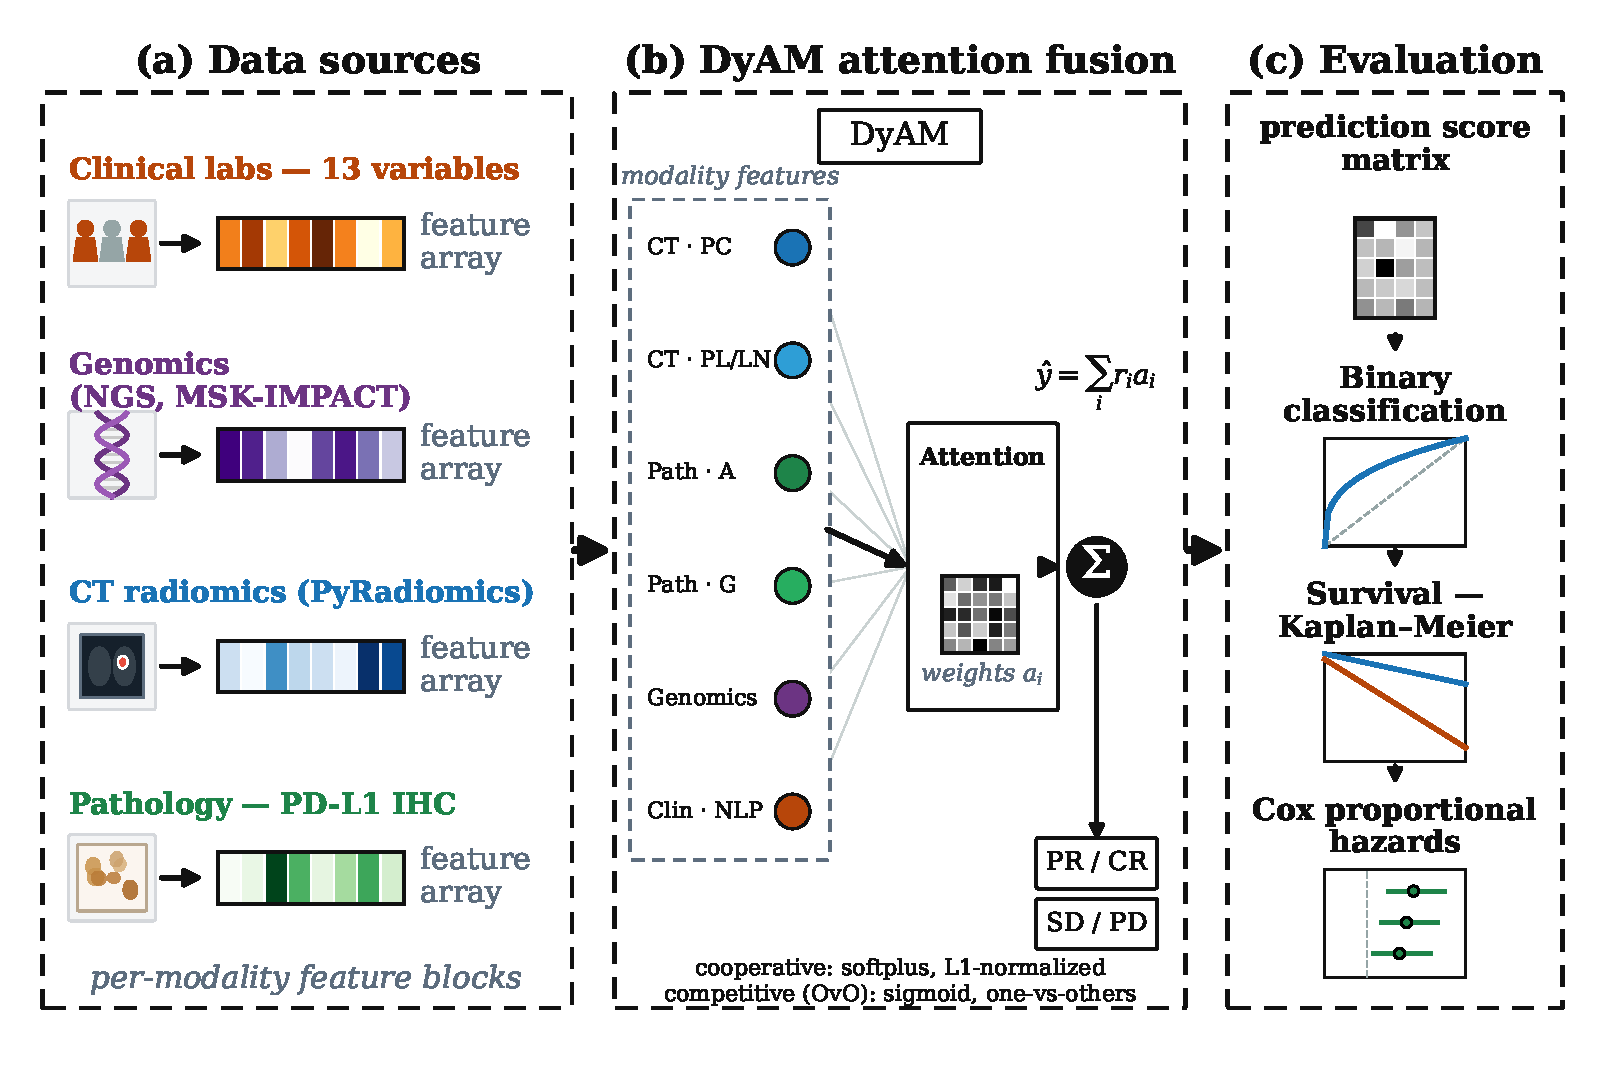
\includegraphics[width=\textwidth]{figures/fig1_overview_demo.pdf}
  \caption{Study overview. (A) The discovery cohort ($n = 247$) and two
    validation cohorts (radiomics-evaluable, $n = 50$; pathology-evaluable,
    $n = 71$) provide six data sources: CT radiomics (modelled separately
    per lesion site: PC, PL, LN), pathology image texture (IHC-A or IHC-G),
    tumour genomics, PD-L1~TPS, and structured clinical variables, giving up
    to seven input modalities per model. (B) The DyAM architecture computes a
    per-modality risk score and combines modalities using either cooperative
    (\texttt{AttentionMatrix}) or competitive one-vs-others
    (\texttt{AttentionMatrixOvO}) attention to produce a fused risk
    prediction $\hat{y}$. (C) Models are evaluated on both binary response
    classification (AUC-ROC with DeLong 95\% CI) and survival endpoints
    (Harrell's C-index, multivariate Cox hazard ratios, and Kaplan--Meier
    log-rank stratification).}
  \label{fig:overview}
\end{figure}

%% ═══════════════════════════════════════════════════════════════════════════
%% B2 — Data Modalities
%% ═══════════════════════════════════════════════════════════════════════════

\subsection{Data Modalities}
\label{sec:modalities}

Six data sources were assembled for each patient
(Table~\ref{tab:modalities}).
Because CT radiomics is modelled separately per lesion site (PC, PL, LN) and
the two pathology feature sets (IHC-A, IHC-G) are used as alternative arms
rather than jointly, a single model receives up to seven input modalities.
CT radiomics features were extracted from baseline scans using the MIRPON
pipeline \cite{Dercle2020} at 1.0~mm isotropic spacing with a window of
$[{-1350}, 250]$~HU, yielding 1{,}688 features per lesion type.
Lesions were categorised by anatomical site:
primary tumour (PC), pleural lesion (PL), and lymph node (LN).
Up to three lesions per site were included, ranked by volume.
Pathology features were derived from PD-L1 immunohistochemistry (IHC) slides:
\emph{IHC-A} comprised 18 pixel-intensity aggregation features
(area, mean intensity, percentiles), while
\emph{IHC-G} comprised 150 grey-level co-occurrence matrix (GLCM)
texture features across six aggregation levels \cite{Vanguri2022}.
Genomic features (11 variables) included tumour mutational burden (TMB) and
the status of eight driver mutations and amplifications derived from
FoundationOne~CDx next-generation sequencing (NGS).
The PD-L1 tumour proportion score (TPS) was obtained from clinical
pathology reports (range 0--100\%).
Clinical laboratory features comprised 13 variables:
age, smoking pack-years, Eastern Cooperative Oncology Group (ECOG)
performance status, serum albumin,
derived neutrophil-to-lymphocyte ratio (dNLR), initial tumour burden,
brain and liver metastasis status, line of therapy, combination therapy,
primary lung site, prior PD-L1 therapy, and adenocarcinoma histology.

For radiomics modalities, features with an intraclass correlation coefficient
(ICC) below 0.15 across test--retest perturbation scans were removed
(robustness filter), and features with a $z$-score exceeding 6 in any patient
were flagged as outliers and excluded.
All modalities except the NLP embedding (Section~\ref{sec:nlp}) were
standardised with \texttt{RobustScaler} (median centring, IQR scaling).
Missing modalities were handled via a binary indicator mask
$\mathbf{m} \in \{0,1\}^N$; masked modalities contribute zero attention and
zero risk to the fused prediction (Section~\ref{sec:model}).

\begin{table}[H]
\caption{Summary of data modalities used in this study.
  All feature counts are post-selection (after ICC and outlier filtering
  for radiomics).
  NLP, natural language processing; GLCM, grey-level co-occurrence matrix;
  IHC, immunohistochemistry; NGS, next-generation sequencing;
  TPS, tumour proportion score.}
\label{tab:modalities}
\small
\begin{tabular}{@{}p{2.3cm}p{2.7cm}p{1.2cm}p{4.1cm}@{}}
\toprule
\textbf{Modality} & \textbf{Source} & \textbf{Features} & \textbf{Clinical meaning} \\
\midrule
CT Radiomics (PC, PL, LN) & MIRPON pipeline & $\leq$1{,}688 & Tumour shape, size, and texture from baseline CT \\
Pathology IHC-A            & PD-L1 IHC slides & 18  & Pixel-intensity aggregation of PD-L1 expression \\
Pathology IHC-G            & PD-L1 IHC slides & 150 & GLCM texture of PD-L1 signal \\
Genomics                   & FoundationOne CDx & 11 & TMB + driver mutation/amplification status \\
PD-L1 TPS                  & Pathology report  & 1  & Tumour proportion score (0--100\%) \\
Clinical labs              & EHR               & 13 & Demographics, performance status, labs \\
\textbf{NLP embedding} (new) & \texttt{all-MiniLM-L6-v2} & 384 & Sentence embedding of clinical lab text \\
\textbf{NLP-PCA16} (new)   & PCA of NLP        & 16  & PCA-compressed NLP (approx.\ 94\% variance) \\
\bottomrule
\end{tabular}
\end{table}

%% ═══════════════════════════════════════════════════════════════════════════
%% B3 — NLP Clinical Embedding
%% ═══════════════════════════════════════════════════════════════════════════

\subsection{NLP Encoding of Tabular Clinical Features}
\label{sec:nlp}

Standard encoding of clinical variables as a 13-dimensional numeric vector
treats each feature independently and loses contextual relationships between
variables (e.g., an elderly patient with low albumin and ECOG~2 implies a
different prognosis than the same values in isolation).
To capture inter-feature context, we converted each patient's clinical
profile into an English-language sentence and extracted a dense semantic
embedding, as illustrated in Figure~\ref{fig:nlp_pipeline}.

\paragraph{Text prompt construction.}
For each patient, the 13 clinical variables were formatted into a structured
natural-language sentence, for example:
\textit{``The patient is a 69-year-old. Smoking history in pack-years is 48.0.
ECOG performance status is 1.0. Blood albumin concentration is 4.00.
Derived neutrophil-to-lymphocyte ratio (dNLR) is 2.40.
Initial tumor burden stands at 52.00.
The patient is diagnosed with adenocarcinoma at the lung site.
Metastatic status: without brain metastasis and without liver metastasis.
Currently undergoing therapy line 2, utilizing combination therapy.
The patient received prior PD-L1 immunotherapy.''}
Binary variables were expanded to descriptive phrases to exploit the
pretrained vocabulary of the encoder.
The full prompt template is provided in Supplementary Note~S1.

\paragraph{Sentence encoder.}
Prompts were encoded with
\texttt{sentence-transformers/all-MiniLM-L6-v2} \cite{Reimers2019,Wang2020MiniLM},
a 6-layer transformer distilled for semantic sentence similarity and
trained on over one billion sentence pairs.
Each patient was represented as a 384-dimensional L2-normalised vector.
No fine-tuning was performed; the model was applied in zero-shot transfer.
We compared this general-purpose encoder against the domain-specific
\texttt{Bio\_ClinicalBERT} \cite{Alsentzer2019};
the domain-specific model performed inferiorly
($\Delta\text{AUC} = -0.017$ versus MiniLM-L6-v2 in the IHC-A arm),
consistent with its design for masked language modelling
rather than sentence-similarity tasks (Supplementary Note~S2).

\paragraph{Dimensionality reduction.}
Principal component analysis (PCA) was applied to the 384-dimensional embeddings,
retaining the top 16 components ($\approx$94\% of variance explained;
Supplementary Figure~S1).
Both the raw 384-dimensional (\emph{NLP raw}) and PCA-compressed
16-dimensional (\emph{NLP-PCA16}) variants were evaluated.
Crucially, the NLP modality was passed to the model with the RobustScaler
disabled (\texttt{no\_scale=True}), as the embeddings are already L2-normalised
and scaling would distort the cosine-similarity geometry of the embedding space.

\begin{figure}[H]
  \centering
  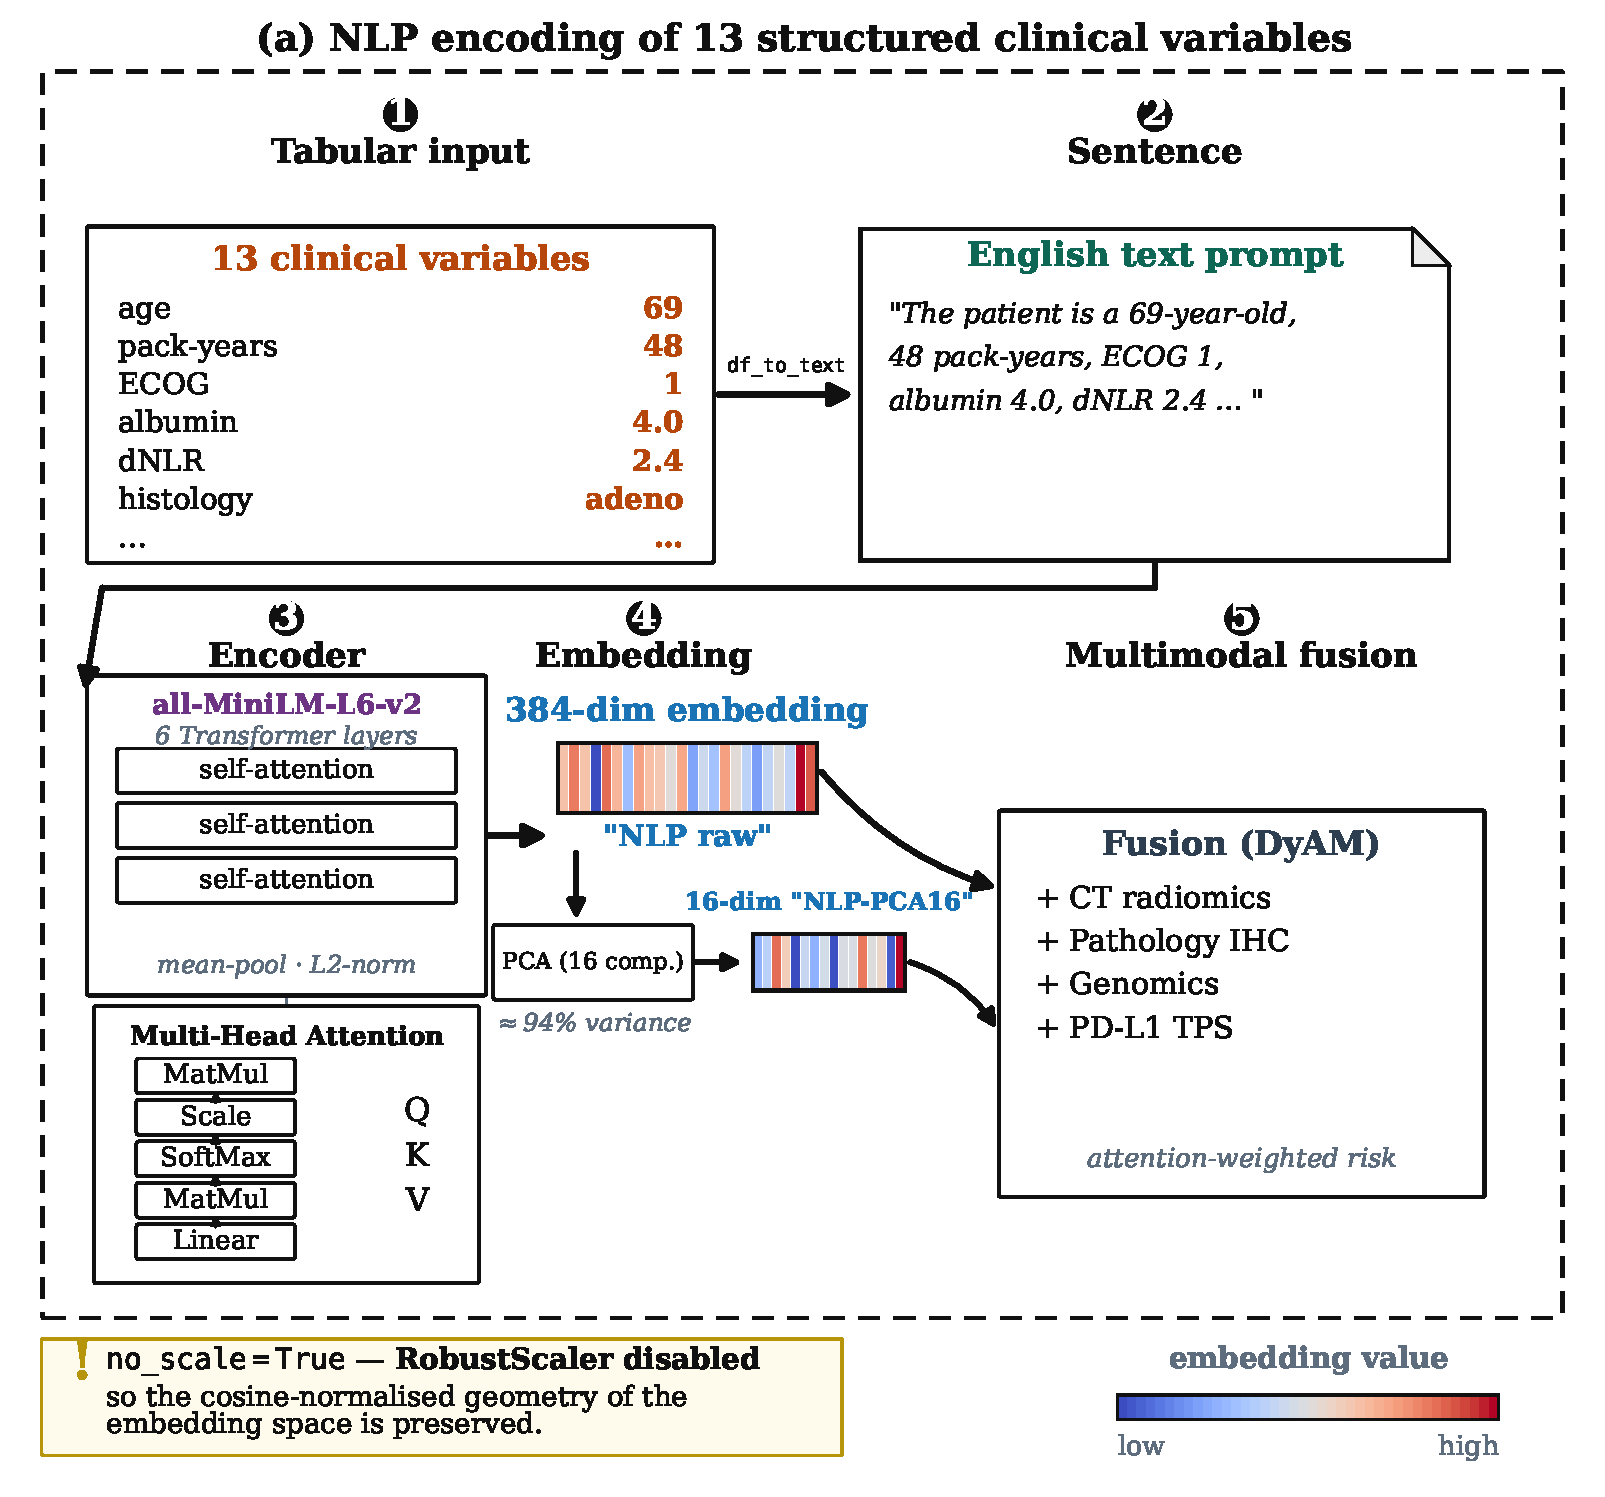
\includegraphics[width=\textwidth]{figures/fig2_nlp_pipeline_demo.pdf}
  \caption{NLP-based encoding of structured clinical features. Thirteen
    numeric clinical variables per patient are converted into a
    natural-language sentence describing the patient's clinical profile
    (example shown), which is then encoded into a 384-dimensional embedding
    using a pretrained sentence transformer (all-MiniLM-L6-v2). The
    384-dimensional embedding (``NLP raw'') is used directly, or further
    reduced to 16 dimensions via PCA (``NLP-PCA16'', retaining
    $\approx$94\% of variance) prior to fusion with other modalities.
    \texttt{no\_scale=True} is applied to NLP embeddings to preserve their
    cosine-normalised geometry.}
  \label{fig:nlp_pipeline}
\end{figure}

%% ═══════════════════════════════════════════════════════════════════════════
%% B4 — Model Architecture
%% ═══════════════════════════════════════════════════════════════════════════

\subsection{Model Architecture}
\label{sec:model}

\paragraph{Dynamic Attention Multimodal (DyAM) model.}
The base model, DyAM \cite{Vanguri2022}, fuses $N$ modalities through
per-modality risk scores and a learned attention mechanism, in the spirit of
attention-based architectures broadly \cite{Vaswani2017}.
Let $\mathbf{x}_i \in \mathbb{R}^{d_i}$ denote the feature vector of
modality~$i$ after optional RobustScaling.
A scalar risk score is computed as:
%
\begin{equation}
  r_i = \tanh\!\left(\mathbf{W}_{\mathrm{r},i}^{\top} \mathbf{x}_i\right),
  \label{eq:risk}
\end{equation}
%
where $\mathbf{W}_{\mathrm{r},i} \in \mathbb{R}^{d_i}$ are learnable weights.
An attention score is produced by an $N \times N$ grid of linear layers
with softplus activation, $\ell_2$-normalised by the modality vector norm:
%
\begin{equation}
  s_i = \frac{\mathrm{softplus}\!\left(\mathbf{W}_{\mathrm{a},ij}^{\top}
        \mathbf{x}_i\right)}{\left\|\mathbf{x}_i\right\|_2}.
  \label{eq:attn_s}
\end{equation}
%
Attention weights are obtained by L1 normalisation across modalities:
%
\begin{equation}
  a_i = \frac{s_i}{\displaystyle\sum_{j=1}^{N} s_j}.
  \label{eq:attn_a}
\end{equation}

\paragraph{OvO competitive attention.}
We propose an alternative attention mechanism inspired by
one-versus-others (OvO) classification \cite{Hastie1998},
in which each modality \emph{competes} against the mean score of
all remaining modalities rather than sharing a fixed budget.
The mean score of the $N-1$ competing modalities is:
%
\begin{equation}
  \mu_{-i} = \frac{1}{N-1} \sum_{j \neq i} s_j,
  \label{eq:ovo_mu}
\end{equation}
%
and the OvO attention score is:
%
\begin{equation}
  \mathrm{ovo}_i = \sigma\!\left(s_i - \mu_{-i}\right),
  \qquad \sigma(z) = (1+e^{-z})^{-1}.
  \label{eq:ovo}
\end{equation}
%
The sigmoid function yields an independent probability that modality~$i$
outperforms the others, rather than a jointly normalised score.
After applying the binary missingness mask $m_i \in \{0,1\}$, the weights
are L1-normalised: $a_i = \mathrm{ovo}_i \cdot m_i \big/
\sum_j \mathrm{ovo}_j \cdot m_j$.
The two attention mechanisms are contrasted schematically in
Figure~\ref{fig:attention_arch}.

\paragraph{Fused prediction and training.}
For both variants, the final risk prediction is:
%
\begin{equation}
  \hat{y} = \sum_{i=1}^{N} r_i \cdot a_i.
  \label{eq:output}
\end{equation}
%
\begin{figure}[H]
  \centering
  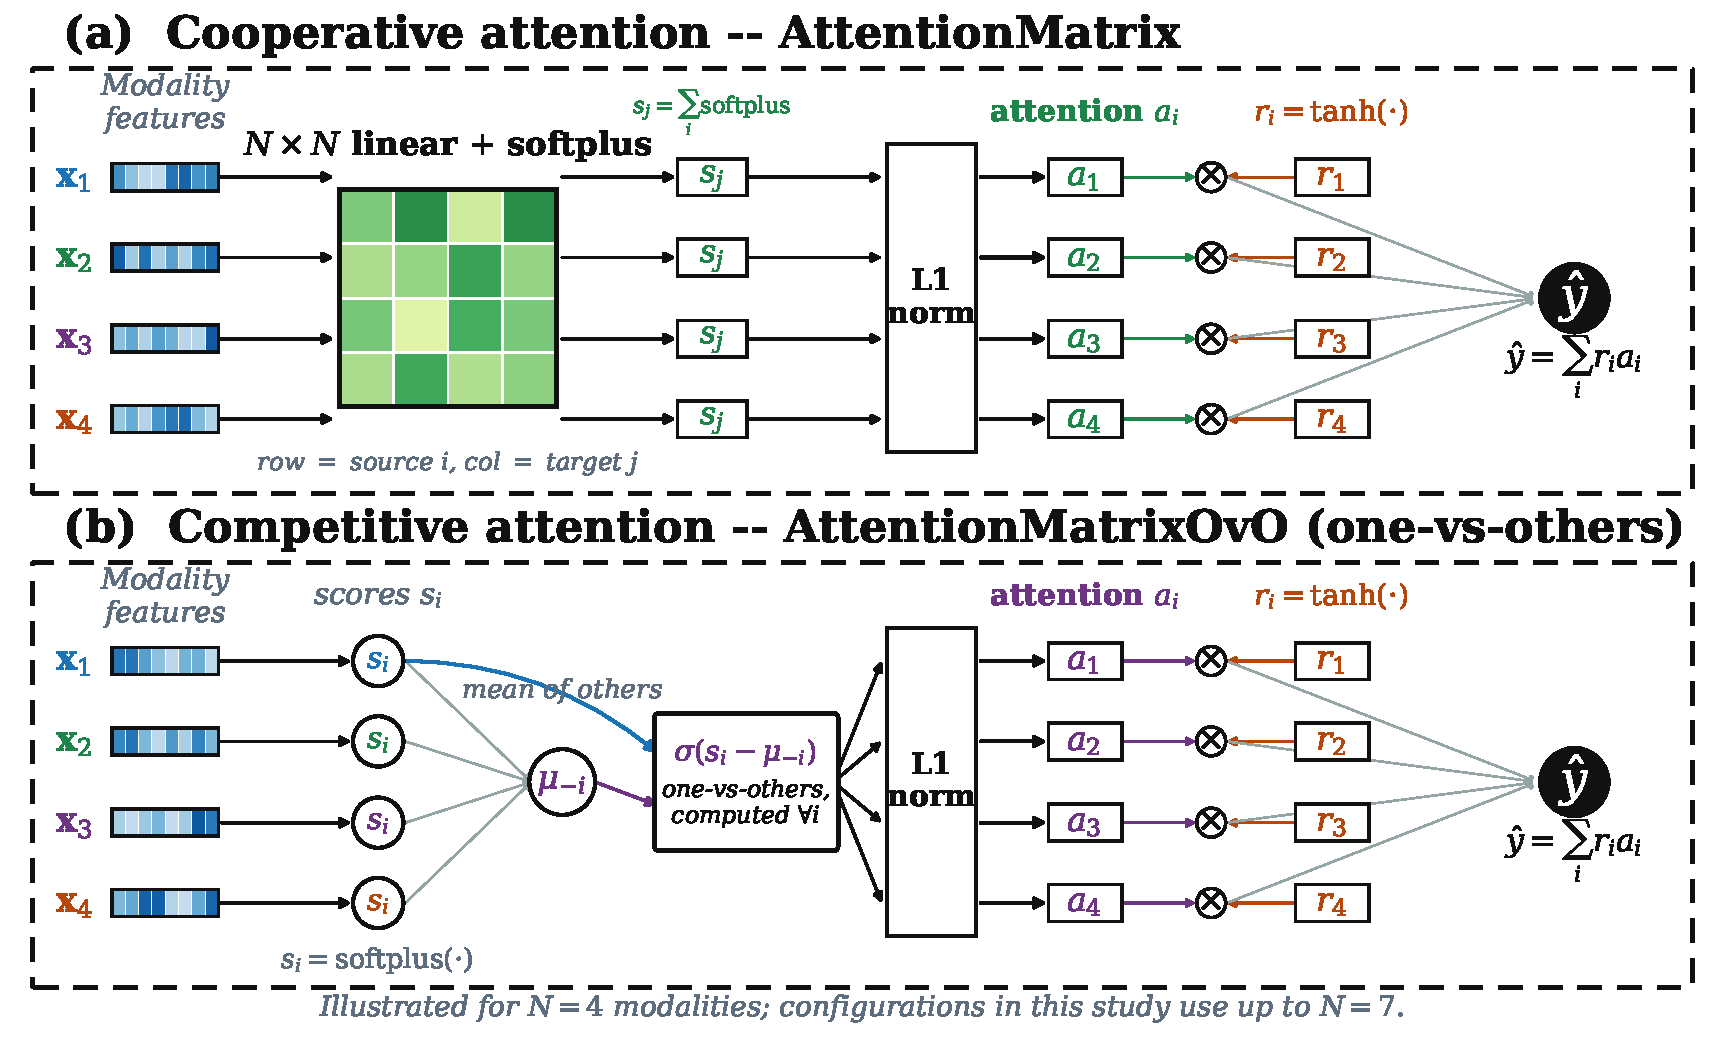
\includegraphics[width=\textwidth]{figures/fig_attention_arch_demo.pdf}
  \caption{Architecture of the two attention mechanisms. Both variants
    compute a per-modality risk score $r_i = \tanh(\mathbf{W}_{r,i}^{\top}
    \mathbf{x}_i)$ (Equation~\ref{eq:risk}) and produce the fused prediction
    $\hat{y} = \sum_i r_i a_i$ (Equation~\ref{eq:output}); they differ only in
    how the attention weights $a_i$ are obtained.
    (A)~\emph{Cooperative} attention (\texttt{AttentionMatrix}): an
    $N\times N$ grid of linear layers with softplus activation produces
    pairwise scores that are column-summed into $s_j$
    (Equation~\ref{eq:attn_s}) and L1-normalised so that the modalities
    share a fixed attention budget (Equation~\ref{eq:attn_a}).
    (B)~\emph{Competitive} one-vs-others attention
    (\texttt{AttentionMatrixOvO}): each modality produces a single score
    $s_i$ that is compared against the mean score of the remaining
    modalities $\mu_{-i}$ through a sigmoid, $\sigma(s_i - \mu_{-i})$
    (Equations~\ref{eq:ovo_mu}--\ref{eq:ovo}), yielding an independent
    competitive weight before L1 normalisation.
    Heatmap bars denote modality feature vectors; the diagram is drawn for
    $N = 4$ modalities for clarity.}
  \label{fig:attention_arch}
\end{figure}

The model was trained with binary cross-entropy loss
(\texttt{BCEWithLogitsLoss}) with automatic inverse-frequency class
weighting to address the $\approx$1:3 class imbalance,
$\ell_1$ regularisation on attention weights ($\alpha = 1.0$),
and $\ell_2$ weight decay ($\beta = 1.0$).
The Adam optimiser was used with a learning rate of 0.01 for 125 epochs.
All experiments used 10-fold stratified cross-validation on the
discovery cohort; predictions were pooled across held-out folds for
AUC computation.

%% ═══════════════════════════════════════════════════════════════════════════
%% B5 — Statistical Analysis
%% ═══════════════════════════════════════════════════════════════════════════

\subsection{Statistical Analysis and Evaluation}
\label{sec:stats}

\paragraph{Discriminative performance.}
Area under the receiver operating characteristic curve (AUC-ROC) was
computed on pooled out-of-fold predictions from 10-fold cross-validation.
Ninety-five percent confidence intervals (CIs) were estimated using the
DeLong structural components method \cite{DeLong1988}.
Two models were considered statistically significantly different when their
95\% CIs did not overlap, consistent with standard practice in oncology
imaging studies.

\paragraph{Survival analysis.}
Harrell's concordance index (C-index) \cite{Harrell1996} was computed from
pooled out-of-fold risk scores against PFS.
Bootstrap 95\% CIs were derived from 1{,}000 resamples with replacement.
For pairwise comparisons, per-fold C-indices (10 values) were compared with
a two-sided Wilcoxon signed-rank test ($\alpha = 0.05$).
Time-dependent AUC was computed at 6, 12, and 18~months using the
cumulative/dynamic estimator \cite{Harrell1996}.
Multivariate Cox proportional hazards regression was fitted with the
DyAM risk score as the primary predictor, adjusted for five clinical
covariates: age, ECOG performance status, serum albumin, dNLR, and
liver metastasis status.
Hazard ratios (HRs) are reported with 95\% CIs and Wald $p$-values.
Model calibration was assessed via the Integrated Brier Score (IBS);
values below 0.25 indicate better-than-random calibration.

\paragraph{Kaplan--Meier survival stratification.}
Patients were dichotomised at risk score~$= 0$, and PFS curves for the
two groups were compared with the log-rank test.
A threshold of $\chi^2 > 7.88$ ($p < 0.005$) was applied as the
significance criterion, consistent with oncology reporting standards.

\paragraph{Software.}
All analyses were performed in Python~3.10 using PyTorch~2.0 (model training),
\texttt{lifelines}~0.27 (Kaplan--Meier, Cox regression, C-index),
\texttt{scikit-survival}~0.21 (time-dependent AUC, Brier score),
and \texttt{scipy}~1.11 (Wilcoxon test).

%% sections/results.tex — Steps B6–B9 + tables
\section{Results}
\label{sec:results}

%% ═══════════════════════════════════════════════════════════════════════════
%% B6 — Multimodal vs Single-Modality Baselines
%% ═══════════════════════════════════════════════════════════════════════════

\subsection{Multimodal Fusion Outperforms Single-Modality Baselines}
\label{sec:baselines}

Within the DyAM framework, models restricted to a single data source
achieved repeated-seed (5~seeds~$\times$~10-fold) AUC values of
$0.616 \pm 0.001$ (TMB), $0.635 \pm 0.021$ (pathology IHC),
$0.673 \pm 0.020$ (CT radiomics), $0.676 \pm 0.013$ (genomics), and
$0.720 \pm 0.012$ (PD-L1~TPS) on the discovery cohort.
PD-L1~TPS was the strongest individual predictor, consistent with its role
as the biomarker in routine clinical use.

Fusing four data sources (CT radiomics, pathology IHC-G, genomics, and
PD-L1~TPS) under the same protocol raised the AUC to $0.760 \pm 0.022$,
exceeding the best single source by $0.040$~AUC; adding NLP-encoded clinical
variables raised it further to $0.783 \pm 0.016$
(Section~\ref{sec:nlp_auc}).
Evaluated on the single cross-validation partition used for the DeLong
confidence intervals reported in Tables~\ref{tab:auc_ihca} and
\ref{tab:auc_ihcg}, the same four-source configuration reached
AUC~$= 0.784$ [95\%~CI: 0.717--0.850] (IHC-G arm;
Table~\ref{tab:auc_ihcg}).
Multimodal fusion is therefore the primary driver of predictive performance
in this cohort, with no individual source approaching the discrimination of
the fused model.

%% ═══════════════════════════════════════════════════════════════════════════
%% B7 — OvO Attention Comparison
%% ═══════════════════════════════════════════════════════════════════════════

\subsection{OvO Competitive Attention Achieves Performance Comparable to Cooperative Attention with a Simpler Parameterization}
\label{sec:ovo}

In an initial exploratory screen across 20 modality configurations
evaluated with a single 10-fold cross-validation partition, the OvO
attention variant outperformed the original cooperative attention
in 7 of 20 cases (35\%), while the original model was superior in 9 of 20
cases (45\%), with 4 identical results (single-modality, where OvO reduces
to the original).
The mean AUC difference was $-0.32\%$ in favour of the original model overall.
The largest single-partition gains for OvO were observed for PDL1+Gen
($\Delta\text{AUC} = +3.27\%$, AUC 0.716 vs.\ 0.693) and Rad+Gen
($\Delta\text{AUC} = +2.23\%$; Table~\ref{tab:ovo}), while the largest
deficits occurred for configurations combining three or more modalities,
particularly when IHC-G or clinical labs were included
(largest deficit: Rad+IHC-A+Gen, $\Delta\text{AUC} = -4.94\%$).

Because a single CV partition can favour either model by chance, we
repeated this comparison as a confirmatory analysis using 5 independent
random partitions (5~seeds~$\times$~10-fold, patient labels re-shuffled per
seed) across the same 21 modality combinations used in the primary
paper-matched configuration set (Section~\ref{sec:baselines}), with paired
bootstrap significance testing on the resulting patient-level scores.
At the primary benchmark configuration (Rad+IHC-G+Gen+PDL1), OvO reached a
repeated-seed mean AUC of $0.773 \pm 0.020$ versus $0.760 \pm 0.022$ for the
original cooperative model ($\Delta\text{AUC} = +0.009$, 95\% bootstrap CI
$[-0.008, 0.027]$, $p = 0.313$); across all four primary benchmarks the two
models differed by at most $0.011$~AUC ($p \geq 0.17$).
Extending the comparison to all 21 modality combinations
(Table~\ref{tab:ovo_all21}), OvO's repeated-seed mean AUC exceeded the
original model's in 12 of 21 configurations and was lower in 5 of 21, with 4
identical (single-modality, where the two formulations coincide
algebraically).
This advantage was concentrated in the many-source regime: for
configurations fusing $k \geq 5$ input sources, OvO matched or exceeded
cooperative attention in 7 of 8 cases (mean $\Delta\text{AUC} = +0.009$,
range $-0.001$ to $+0.018$), whereas for $k = 2$--$4$ it led in only 5 of 9
cases with a far wider spread (mean $+0.003$, range $-0.028$ to $+0.045$).
Notably, this is the opposite of the pattern suggested by the
single-partition screen, which had favoured OvO at low modality counts;
the repeated-seed evaluation instead places OvO's small but consistent edge
in precisely the multi-source configurations the fusion model is intended
for.
These per-$k$ counts are descriptive: formal significance testing was
performed only at the four primary benchmarks, and the effect sizes involved
($\leq 0.018$~AUC) remain below the seed-to-seed standard deviation
($\approx 0.02$), so the trend should be read as a consistency pattern
rather than a demonstrated superiority.
The single-partition ``best-performing configuration'' identified in the
initial screen (OvO Rad+IHC-G+Gen+PDL1, AUC~$=0.8003$ [95\%~CI:
0.739--0.862]) illustrates how favourable a single partition can be: the
same configuration's repeated-seed mean AUC was $0.773$, and OvO's rank
relative to the cooperative model reversed once averaged across seeds.

As a further robustness check, we combined OvO attention with the
NLP-clinical encoding described in Section~\ref{sec:nlp_auc}, repeating the
same 21-combination, 5-seed evaluation with clinical text embeddings added
to each configuration.
OvO+NLP reproduced the same fusion-dependent improvement pattern observed
in the primary NLP-clinical analysis (Section~\ref{sec:nlp_auc}): AUC
improved relative to the no-clinical baseline in 15 of 21 configurations
(an identical set of configurations), and declined in the same six single-
or near-single-modality configurations where any clinical addition diluted
a strong standalone signal (PD-L1, radiomics-only, and similar).
At the primary benchmark, OvO+NLP reached a repeated-seed mean
AUC~$=0.782 \pm 0.017$, matching the $0.783 \pm 0.016$ obtained by the
repeated-seed NLP-clinical confirmation at the same configuration
(Section~\ref{sec:nlp_auc}).
Under the single-partition protocol, OvO+NLP reached AUC~$=0.8133$ at the
Rad+IHC-A+Gen+TMB+PDL1 configuration, the highest value obtained under
either evaluation protocol in this study.
This shows that OvO's simpler, $N$-parameter formulation (independent
per-modality scores compared against the mean of the others) delivers the
same NLP-clinical benefit as the cooperative model without the
$N \times N$ weight matrix, and that the clinical-encoding intervention,
not the choice of attention mechanism, is the source of that gain.
Table~\ref{tab:ovo} summarises the exploratory single-partition screen and
Table~\ref{tab:ovo_all21} gives the repeated-seed AUC of all three models
across all 21 configurations; the corresponding single-partition values are
provided in Supplementary Table~S3.


\begin{table}[H]
\caption{Top configurations from the exploratory, single-partition screen
  comparing OvO competitive attention and original cooperative attention.
  $\Delta$AUC is computed as OvO minus Original.
  Bold denotes the higher AUC for each row.
  As described in the text, these single-partition differences were not
  reproducible under repeated-seed evaluation (Table~\ref{tab:ovo_all21})
  and should be interpreted as an initial screen rather than a confirmed
  effect.
  Gen, genomics; Rad, CT radiomics; IHC-A/G, immunohistochemistry variants;
  PDL1, PD-L1 TPS score.}
\label{tab:ovo}
\begin{minipage}[t]{0.48\textwidth}
\centering
\footnotesize
\textit{OvO better ($\Delta > 0$)}\\[3pt]
\begin{tabular}{@{}p{2.5cm}ccc@{}}
\toprule
Configuration & Orig. & OvO & $\Delta$ \\
\midrule
PDL1+Gen           & 0.693 & \textbf{0.716} & +3.27\% \\
Rad+Gen            & 0.738 & \textbf{0.755} & +2.23\% \\
Rad+IHC-G+Gen+PDL1 & 0.784 & \textbf{0.800} & +2.10\% \\
Rad+IHC-A+Gen+PDL1 & 0.764 & \textbf{0.777} & +1.63\% \\
TMB+PDL1           & 0.705 & \textbf{0.715} & +1.42\% \\
\bottomrule
\end{tabular}
\end{minipage}
\hfill
\begin{minipage}[t]{0.48\textwidth}
\centering
\footnotesize
\textit{Original better ($\Delta < 0$)}\\[3pt]
\begin{tabular}{@{}p{2.5cm}ccc@{}}
\toprule
Configuration & Orig. & OvO & $\Delta$ \\
\midrule
Rad+IHC-A+Gen      & \textbf{0.757} & 0.719 & $-4.94\%$ \\
IHC-G+Gen          & \textbf{0.756} & 0.723 & $-4.33\%$ \\
Rad+IHC-A+Gen+PDL1+Labs & \textbf{0.768} & 0.747 & $-2.83\%$ \\
Rad+IHC-G+Gen      & \textbf{0.787} & 0.766 & $-2.66\%$ \\
Rad+IHC-G+Gen+PDL1+Labs & \textbf{0.788} & 0.783 & $-0.56\%$ \\
\bottomrule
\end{tabular}
\end{minipage}
\end{table}

\begin{table}[H]
\centering
\caption{Repeated-seed (5~seeds~$\times$~10-fold) AUC across all 21
  paper-matched modality combinations, for the original cooperative
  attention (DyAM), OvO competitive attention, and OvO combined with
  NLP-clinical encoding. $k$ is the number of fused input sources
  (CT radiomics contributes one source per lesion site).
  Bold marks the highest value in each row. For $k = 1$ OvO reduces
  algebraically to the cooperative formulation, hence the identical values.
  Configurations 8, 11, 18 and 21 are the primary benchmarks BM4, BM3, BM1
  and BM2; paired-bootstrap testing (2000 resamples) was performed at those
  four only, giving $\Delta\text{AUC}$ (OvO $-$ DyAM) of $+0.011$
  [$-0.005$, $0.026$], $p = 0.172$ (BM4); $+0.000$ [$-0.012$, $0.013$],
  $p = 0.980$ (BM3); $+0.009$ [$-0.008$, $0.027$], $p = 0.313$ (BM1); and
  $-0.004$ [$-0.020$, $0.009$], $p = 0.536$ (BM2).
  Single-partition values for the same 21 configurations are given in
  Supplementary Table~S3.}
\label{tab:ovo_all21}
\footnotesize
\begin{tabular}{@{}rlcccc@{}}
\toprule
\# & Configuration & $k$ & DyAM & OvO & OvO+NLP \\
\midrule
1  & TMB                              & 1 & \textbf{0.616} & \textbf{0.616} & 0.606 \\
2  & PDL1                             & 1 & \textbf{0.720} & \textbf{0.720} & 0.694 \\
3  & IHC-A                            & 1 & \textbf{0.635} & \textbf{0.635} & 0.625 \\
4  & Gen                              & 1 & \textbf{0.676} & \textbf{0.676} & 0.661 \\
5  & Rad                              & 3 & \textbf{0.673} & 0.659 & 0.651 \\
6  & Rad-LU                           & 4 & 0.637 & \textbf{0.646} & 0.629 \\
7  & TMB+PDL1                         & 2 & 0.664 & 0.709 & \textbf{0.714} \\
8  & PDL1+Gen (BM4)                   & 2 & 0.707 & 0.718 & \textbf{0.747} \\
9  & Rad+IHC-A                        & 4 & 0.671 & 0.668 & \textbf{0.712} \\
10 & Rad+IHC-G                        & 4 & 0.706 & 0.703 & \textbf{0.736} \\
11 & Rad+Gen (BM3)                    & 4 & 0.709 & \textbf{0.713} & 0.708 \\
12 & IHC-A+Gen                        & 2 & 0.693 & 0.697 & \textbf{0.702} \\
13 & IHC-G+Gen                        & 2 & 0.747 & 0.719 & \textbf{0.752} \\
14 & Rad+IHC-A+Gen                    & 5 & 0.725 & 0.735 & \textbf{0.744} \\
15 & Rad+IHC-G+Gen                    & 5 & 0.751 & 0.752 & \textbf{0.760} \\
16 & Rad+IHC-A+MutAmp                 & 6 & 0.734 & 0.744 & \textbf{0.747} \\
17 & Rad+IHC-A+Gen+PDL1               & 6 & 0.743 & 0.753 & \textbf{0.757} \\
18 & Rad+IHC-G+Gen+PDL1 (BM1)         & 6 & 0.760 & 0.773 & \textbf{0.782} \\
19 & Rad+IHC-A+Gen+TMB+PDL1           & 7 & 0.749 & \textbf{0.766} & 0.765 \\
20 & Rad+IHC-A+Gen+PDL1+Labs          & 7 & 0.736 & 0.745 & \textbf{0.757} \\
21 & Rad+IHC-G+Gen+PDL1+Labs (BM2)    & 7 & 0.764 & 0.763 & \textbf{0.782} \\
\bottomrule
\end{tabular}
\end{table}

%% ═══════════════════════════════════════════════════════════════════════════
%% B8 — NLP AUC Analysis
%% ═══════════════════════════════════════════════════════════════════════════

\subsection{NLP Encoding Consistently Improves AUC over Numeric Clinical Features}
\label{sec:nlp_auc}

Seven NLP encoding variants were evaluated against numeric clinical labs
as a reference.
In the IHC-A arm, NLP-PCA16 achieved the highest AUC among clinical
encoding strategies (AUC~$= 0.784$, 95\%~CI: 0.719--0.848;
$\Delta\text{AUC} = +0.020$ over no-clinical baseline),
compared to $+0.004$ for numeric labs (Table~\ref{tab:auc_ihca}).
In the IHC-G arm, NLP raw (384-dimensional) achieved the best result
(AUC~$= 0.813$, 95\%~CI: 0.753--0.874; $\Delta\text{AUC} = +0.030$),
with NLP-PCA16 performing comparably ($\Delta\text{AUC} = +0.028$;
Table~\ref{tab:auc_ihcg}). These results are visualised in
Figure~\ref{fig:auc_comparison}.

However, all pairwise DeLong confidence intervals overlapped substantially,
meaning no individual NLP variant reached statistical significance compared
to the no-clinical baseline.
The largest separation was observed in the IHC-G arm
(NLP raw vs.\ no-clinical: lower CI 0.753 vs.\ upper CI 0.850;
overlap $\approx$0.10).
As discussed in Section~\ref{sec:discussion}, this is attributable to
the limited cohort size ($n = 247$) rather than an absent effect.

\emph{Repeated-seed confirmation.}
To verify that the advantage of NLP encoding is not specific to a single
CV partition, we repeated the NLP-versus-labs comparison under the
repeated-seed protocol of Section~\ref{sec:ovo} (5~seeds~$\times$~10-fold)
across all 21 paper-matched modality combinations, using masked averaging
of the per-modality risk scores as the fusion rule to isolate the encoding
effect from attention learning.
NLP encoding exceeded numeric labs in 19 of 21 combinations; the two
exceptions (PD-L1 alone and the four-lesion radiomics-only configuration)
are single-source configurations in which adding any clinical modality
dilutes a strong standalone signal.
At the primary IHC-G-arm configuration (Rad+IHC-G+Gen+PDL1), repeated-seed
mean AUC was $0.766 \pm 0.013$ with numeric labs versus
$0.783 \pm 0.016$ with NLP encoding ($\Delta = +0.017$); the corresponding
IHC-A-arm values were $0.742 \pm 0.014$ versus $0.758 \pm 0.013$
($\Delta = +0.016$).
The same NLP gain also held under OvO attention
(Section~\ref{sec:ovo}), indicating the improvement is robust to both the
CV partition and the fusion mechanism.

\emph{Domain-specific versus general-purpose encoder.}
Bio\_ClinicalBERT \cite{Alsentzer2019}, PCA-compressed to 16 dimensions,
performed below MiniLM-L6-v2 in the IHC-A arm
(AUC~$= 0.767$ versus $0.784$; $\Delta\text{AUC} = -0.017$),
consistent with its pretraining objective of masked language modelling
on clinical notes rather than semantic sentence similarity.

\emph{Combined encoding.}
Concatenating numeric labs and NLP-PCA16 as separate modalities
(8 modalities total) degraded performance
(AUC~$= 0.753$, $\Delta = -0.011$ in IHC-A),
likely due to unstable attention learning with $n/N = 247/8 \approx 31$.
NLP encoding is therefore recommended as a \emph{replacement} for,
rather than an addition to, numeric clinical features.

%% tables/table2_auc_ihca.tex
\begin{table}[H]
\caption{AUC comparison across clinical encoding strategies --- IHC-A arm.
  All models use the DyAM architecture with CT radiomics (PC, PL, LN),
  pathology IHC-A, genomics, and PD-L1~TPS as base modalities;
  clinical encoding is the varied factor.
  AUC computed on pooled out-of-fold predictions from 10-fold
  cross-validation ($n = 247$).
  95\%~CI by DeLong structural components method.
  $\Delta$AUC relative to the no-clinical baseline.
  $^\dagger$Best-performing NLP variant; n/a, not applicable.
  NLP, natural language processing; PCA, principal component analysis.}
\label{tab:auc_ihca}
\begin{tabular}{lccc}
\toprule
\textbf{Model} & \textbf{AUC} & \textbf{95\%~CI} & \boldmath{$\Delta$}\textbf{AUC} \\
\midrule
No clinical (baseline)        & 0.764 & [0.695--0.833] & (ref) \\
+ Labs (13-dim numeric)       & 0.768 & [0.700--0.837] & $+0.004$ \\
+ NLP raw (384-dim)           & 0.781 & [0.717--0.845] & $+0.017$ \\
\textbf{+ NLP-PCA16 (16-dim)}\textsuperscript{$\dagger$}
                              & \textbf{0.784} & \textbf{[0.719--0.848]} & $\mathbf{+0.020}$ \\
+ Labs + NLP (combined)       & 0.767 & [0.700--0.835] & $+0.003$ \\
+ Labs + NLP-PCA16 (combined) & 0.753 & [0.682--0.823] & $-0.011$ \\
+ BioClinBERT-PCA16           & 0.767 & [0.701--0.833] & $+0.003$ \\
\bottomrule
\end{tabular}
\end{table}

%% tables/table3_auc_ihcg.tex
\begin{table}[H]
\caption{AUC comparison across clinical encoding strategies --- IHC-G arm.
  Base modalities: CT radiomics (PC, PL, LN), pathology IHC-G (GLCM texture),
  genomics, and PD-L1~TPS.
  All other details as in Table~\ref{tab:auc_ihca}.
  $^\dagger$Best-performing NLP variant and overall best model.}
\label{tab:auc_ihcg}
\begin{tabular}{lccc}
\toprule
\textbf{Model} & \textbf{AUC} & \textbf{95\%~CI} & \boldmath{$\Delta$}\textbf{AUC} \\
\midrule
No clinical (baseline)  & 0.784 & [0.717--0.850] & (ref) \\
+ Labs (13-dim numeric) & 0.788 & [0.723--0.853] & $+0.004$ \\
\textbf{+ NLP raw (384-dim)}\textsuperscript{$\dagger$}
                        & \textbf{0.813} & \textbf{[0.753--0.874]} & $\mathbf{+0.030}$ \\
+ NLP-PCA16 (16-dim)    & 0.812 & [0.751--0.873] & $+0.028$ \\
\bottomrule
\end{tabular}
\end{table}


\begin{figure}[H]
  \centering
  \subfloat[IHC-A arm (7 variants)\label{fig:auc_ihca}]{%
    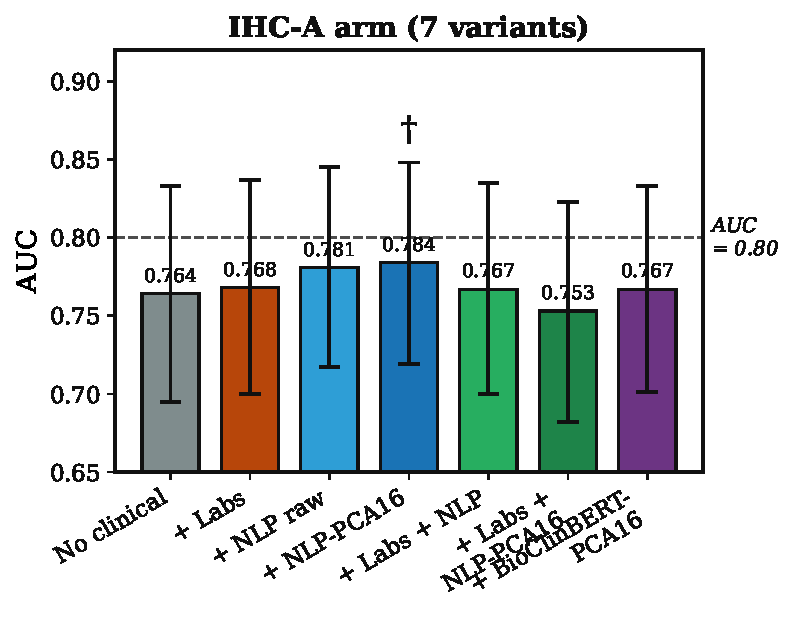
\includegraphics[width=0.48\textwidth]{figures/fig3a_auc_ihca_demo.pdf}}
  \hfill
  \subfloat[IHC-G arm (4 variants)\label{fig:auc_ihcg}]{%
    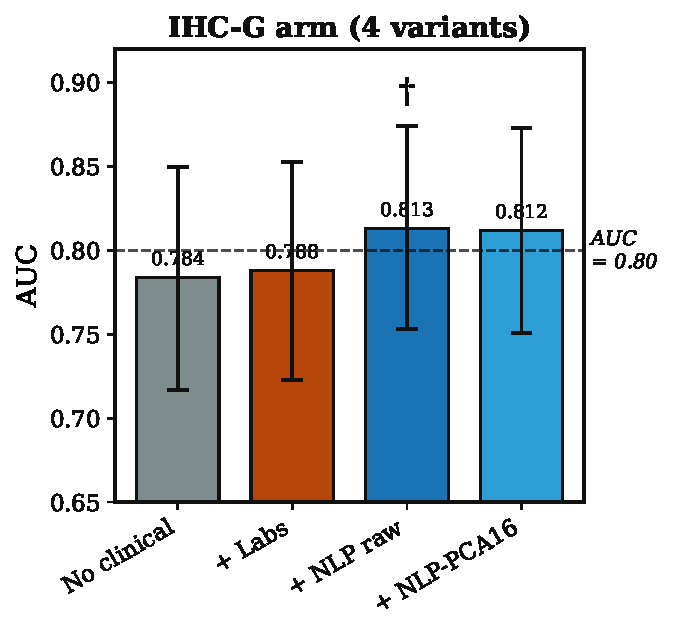
\includegraphics[width=0.48\textwidth]{figures/fig3b_auc_ihcg_demo.pdf}}
  \caption{AUC comparison across clinical encoding strategies for
    (\textbf{A}) the IHC-A arm and (\textbf{B}) the IHC-G arm. Bars show
    pooled out-of-fold AUC from 10-fold cross-validation ($n = 247$); error
    bars denote DeLong 95\% confidence intervals. The dashed horizontal line
    at AUC~$=0.80$ indicates the conventional threshold for clinically
    useful discrimination. $^\dagger$Best-performing model overall (DyAM
    Rad+IHC-G+Gen+PDL1+NLP raw, AUC~$=0.813$).}
  \label{fig:auc_comparison}
\end{figure}

%% ═══════════════════════════════════════════════════════════════════════════
%% B9 — Survival Analysis
%% ═══════════════════════════════════════════════════════════════════════════

\subsection{Survival Analysis: NLP Encoding Enhances Independent Prognostic Value}
\label{sec:survival}

The DyAM risk score was a statistically significant independent prognostic
factor for PFS across all eight model variants in multivariate Cox regression
(all $p < 0.001$, adjusted for age, ECOG performance status, serum albumin,
dNLR, and liver metastasis status; Table~\ref{tab:survival}).

\paragraph{Cox hazard ratios.}
NLP-PCA16 yielded the highest hazard ratio in the IHC-A arm
(HR~$= 6.07$, 95\%~CI: 3.50--10.52), compared with HR~$= 5.30$
[3.10--9.07] for the no-clinical baseline and HR~$= 5.31$ [2.88--9.79]
for numeric labs.
In the IHC-G arm, NLP raw achieved HR~$= 4.97$ [2.98--8.31] versus
HR~$= 4.74$ [2.82--7.97] for no-clinical and
HR~$= 4.49$ [2.56--7.89] for numeric labs.
Notably, numeric labs did not improve the hazard ratio in either arm,
whereas NLP encoding consistently increased it, suggesting that
sentence-embedded clinical context captures prognostic information
not represented by the five Cox covariates or by raw numeric features.

\paragraph{Time-dependent AUC.}
The advantage of NLP encoding was time-dependent:
in the IHC-A arm, NLP-PCA16 improved time-dependent AUC
by $+0.024$ at 12~months and $+0.020$ at 18~months relative to the
no-clinical baseline, with smaller differences at 6~months ($+0.002$).
This pattern, concentrated at late timepoints, is consistent with the
hypothesis that sentence embeddings primarily encode long-term
survival characteristics rather than short-term binary response.

\paragraph{C-index.}
Harrell's C-index showed a consistent but modest improvement with
NLP variants ($\Delta C = +0.005$ in both IHC arms;
Wilcoxon $p = 0.492$ and $p = 0.375$ for IHC-A and IHC-G, respectively),
which did not reach statistical significance.
The high inter-fold variance (range 0.52--0.78 across 10 folds)
and the small fold size ($\approx$25 patients per fold) explain the
non-significant result independently of the true effect size.

\paragraph{Calibration.}
All models were well-calibrated, with Integrated Brier Scores of
0.172--0.175, well below the 0.25 random-classifier baseline.
NLP-PCA16 in the IHC-A arm achieved the lowest IBS (0.1716),
indicating marginally superior probabilistic calibration.

\paragraph{Kaplan--Meier stratification.}
Dichotomising patients at risk score~$=0$ produced statistically significant
separation between high- and low-risk groups for all eight models
($p < 0.005$ by log-rank test; Table~\ref{tab:km}), with the highest
$\chi^2$ statistic observed for the IHC-G arm with NLP raw clinical encoding
($\chi^2 = 28.92$). Representative curves are shown in
Figure~\ref{fig:km_curves}, and a summary of all survival metrics is shown
in Figure~\ref{fig:survival_summary}.

%% tables/table4_survival.tex
\begin{table}[H]
\caption{Survival analysis results across all model variants.
  Discovery cohort ($n = 247$; 209 events, 84.6\%; median PFS 2.7~months).
  C-index: Harrell's concordance index with bootstrap 95\%~CI (1{,}000
  resamples). Cox HR: hazard ratio from multivariate Cox proportional
  hazards regression adjusted for age, ECOG, albumin, dNLR, and liver
  metastases (95\%~CI; Wald $p$-value). tdAUC: time-dependent AUC at
  12~months. IBS: Integrated Brier Score (lower is better;
  $< 0.25$ indicates better-than-random calibration).
  All Cox $p < 0.001$.
  Bold: best value per column within each IHC arm.}
\label{tab:survival}
\small
\begin{tabular}{@{}p{3.4cm}ccccc@{}}
\toprule
\textbf{Model} &
\textbf{C-index} & \textbf{[95\%~CI]} &
\textbf{Cox HR} & \textbf{[95\%~CI]} &
\textbf{IBS} \\
\midrule
\multicolumn{6}{l}{\textit{IHC-A arm}} \\
No clinical          & 0.623 & [0.580--0.665] & 5.30 & [3.10--9.07]   & 0.1745 \\
+ Labs               & 0.626 & [0.583--0.669] & 5.31 & [2.88--9.79]   & 0.1739 \\
+ NLP raw            & 0.625 & [0.583--0.663] & 5.91 & [3.40--10.25]  & 0.1723 \\
\textbf{+ NLP-PCA16} & \textbf{0.628} & \textbf{[0.584--0.668]}
                     & \textbf{6.07} & \textbf{[3.50--10.52]}
                     & \textbf{0.1716} \\
\midrule
\multicolumn{6}{l}{\textit{IHC-G arm}} \\
No clinical          & 0.626 & [0.583--0.665] & 4.74 & [2.82--7.97]  & 0.1748 \\
+ Labs               & \textbf{0.632} & \textbf{[0.587--0.675]} & 4.49 & [2.56--7.89]  & 0.1746 \\
\textbf{+ NLP raw}   & \textbf{0.632} & \textbf{[0.591--0.672]}
                     & \textbf{4.97} & \textbf{[2.98--8.31]}
                     & \textbf{0.1736} \\
+ NLP-PCA16          & 0.631 & [0.590--0.672] & 4.69 & [2.86--7.68]  & 0.1736 \\
\bottomrule
\end{tabular}
\end{table}

%% tables/table5_km.tex
\begin{table}[H]
\caption{Kaplan--Meier log-rank statistics for survival stratification.
  Patients were dichotomised at risk score~$= 0$.
  Threshold for significance: $\chi^2 > 7.88$ ($p < 0.005$).
  All models achieve $p < 0.005$.
  $\star$ Highest $\chi^2$ across all tested models.}
\label{tab:km}
\begin{tabular}{llcc}
\toprule
\textbf{Model} & \textbf{IHC arm} & \boldmath{$\chi^2$} & \textbf{$p$-value} \\
\midrule
DyAM No clinical & IHC-A & 28.17 & $< 0.005$ \\
DyAM + NLP-PCA16 & IHC-A & 23.74 & $< 0.005$ \\
DyAM No clinical & IHC-G & 20.07 & $< 0.005$ \\
\textbf{DyAM + NLP-PCA16} & \textbf{IHC-G} & \textbf{28.92}$^{\star}$ & $\mathbf{< 0.005}$ \\
\bottomrule
\end{tabular}
\end{table}


\begin{figure}[H]
  \centering
  \subfloat[IHC-A, no clinical ($\chi^2 = 28.17$)]{%
    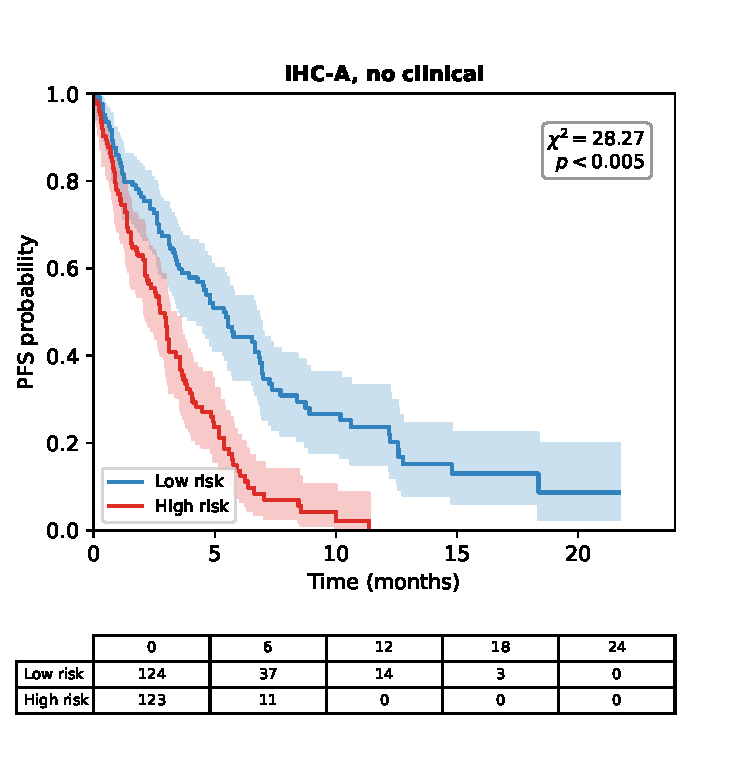
\includegraphics[width=0.48\textwidth]{figures/fig4a_km_ihca_noclin.pdf}}
  \hfill
  \subfloat[IHC-A, + NLP-PCA16 ($\chi^2 = 23.74$)]{%
    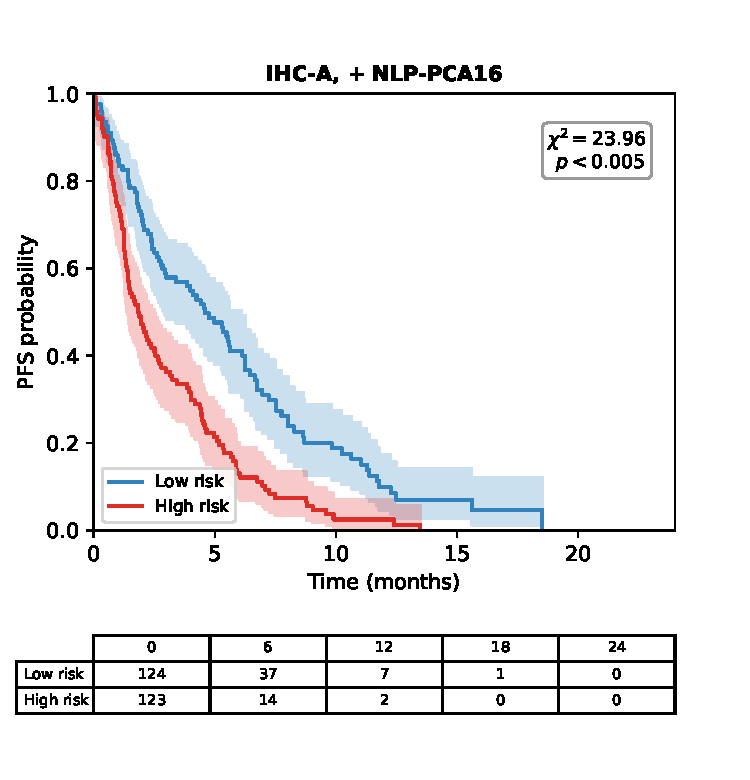
\includegraphics[width=0.48\textwidth]{figures/fig4b_km_ihca_nlppca16.pdf}}

  \subfloat[IHC-G, no clinical ($\chi^2 = 20.07$)]{%
    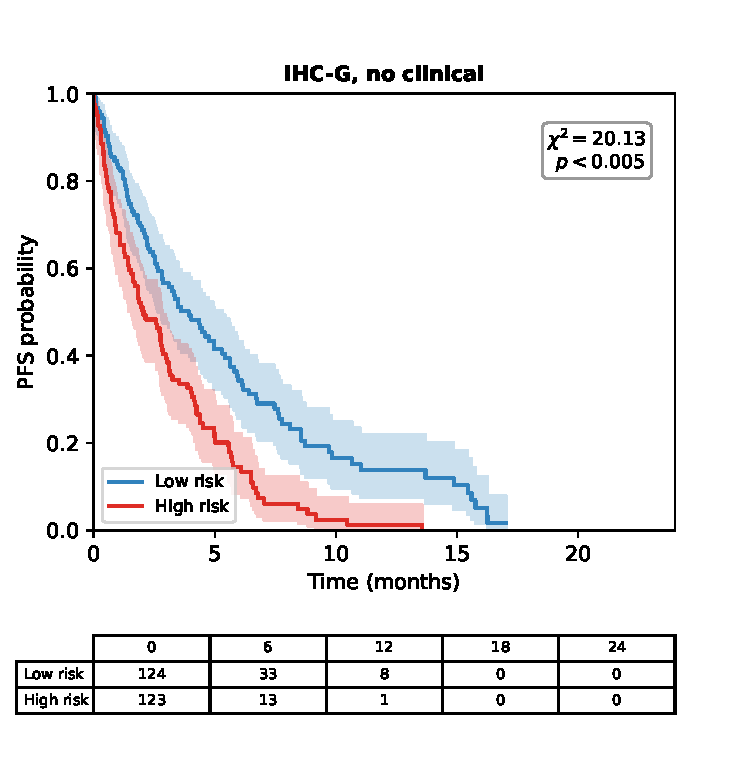
\includegraphics[width=0.48\textwidth]{figures/fig4c_km_ihcg_noclin.pdf}}
  \hfill
  \subfloat[IHC-G, + NLP raw ($\chi^2 = 28.92^{\star}$)]{%
    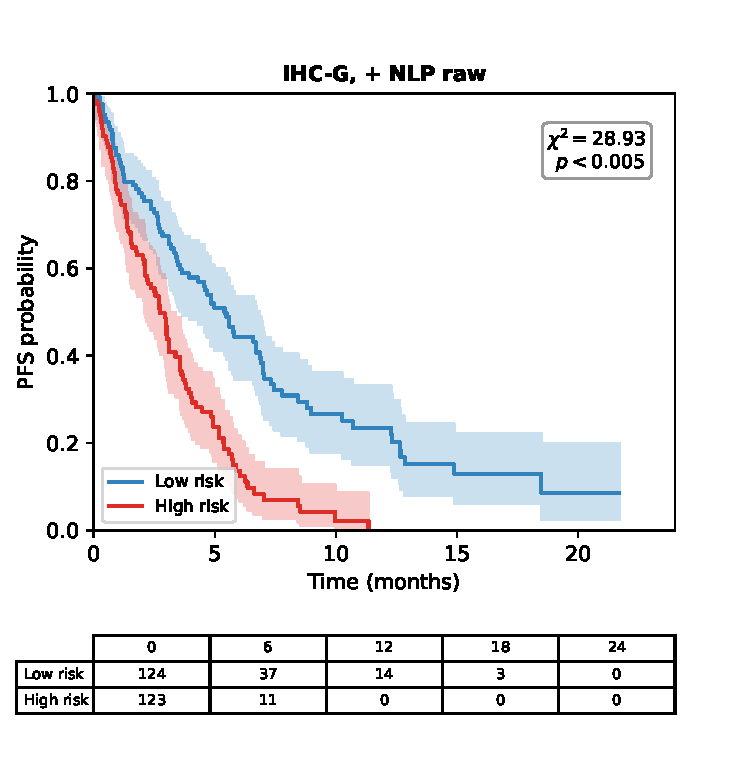
\includegraphics[width=0.48\textwidth]{figures/fig4d_km_ihcg_nlpraw.pdf}}
  \caption{Kaplan--Meier progression-free survival curves for representative
    models, stratified at risk score~$=0$ into high-risk (red) and low-risk
    (blue) groups, with number-at-risk tables.
    (\textbf{A}) IHC-A arm, no clinical encoding.
    (\textbf{B}) IHC-A arm with NLP-PCA16 clinical encoding.
    (\textbf{C}) IHC-G arm, no clinical encoding.
    (\textbf{D}) IHC-G arm with NLP raw clinical encoding
    ($^{\star}$the highest log-rank statistic among all tested models).
    All comparisons reach $p < 0.005$ by the log-rank test.}
  \label{fig:km_curves}
\end{figure}

\begin{figure}[H]
  \centering
  \subfloat[Harrell's C-index (bootstrap 95\% CI)]{%
    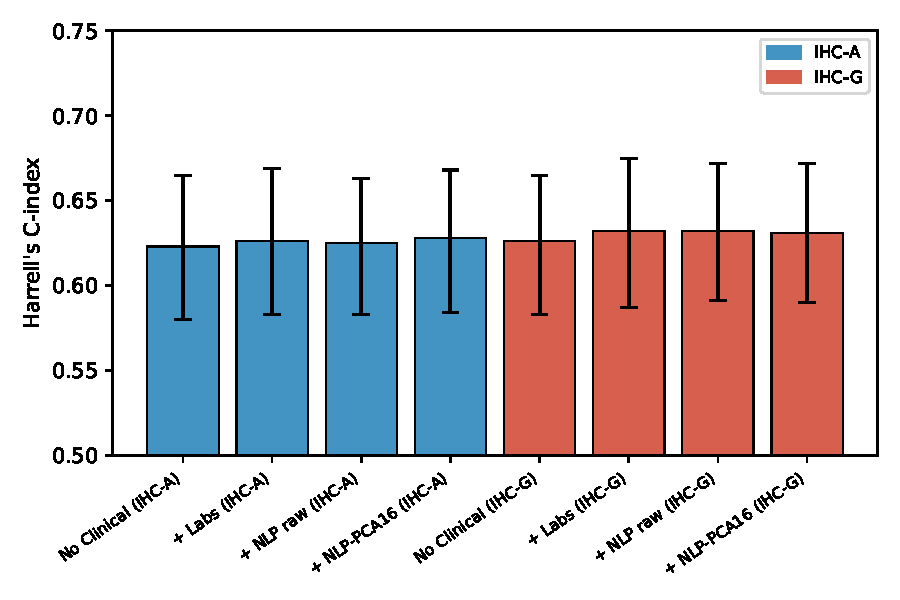
\includegraphics[width=0.48\textwidth]{figures/fig5a_cindex.pdf}}
  \hfill
  \subfloat[Time-dependent AUC (6/12/18~months)]{%
    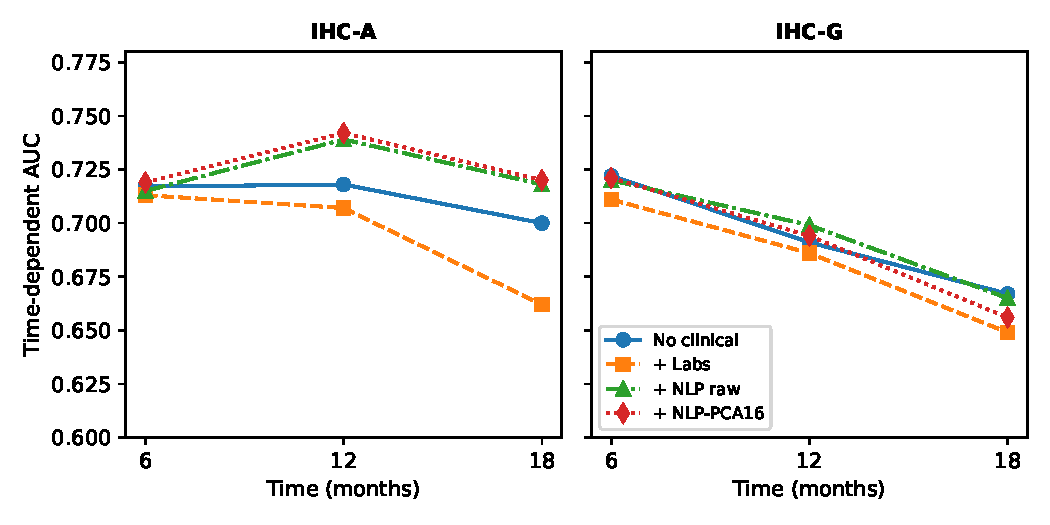
\includegraphics[width=0.48\textwidth]{figures/fig5b_tdauc.pdf}}

  \subfloat[Multivariate Cox hazard ratios (forest plot)]{%
    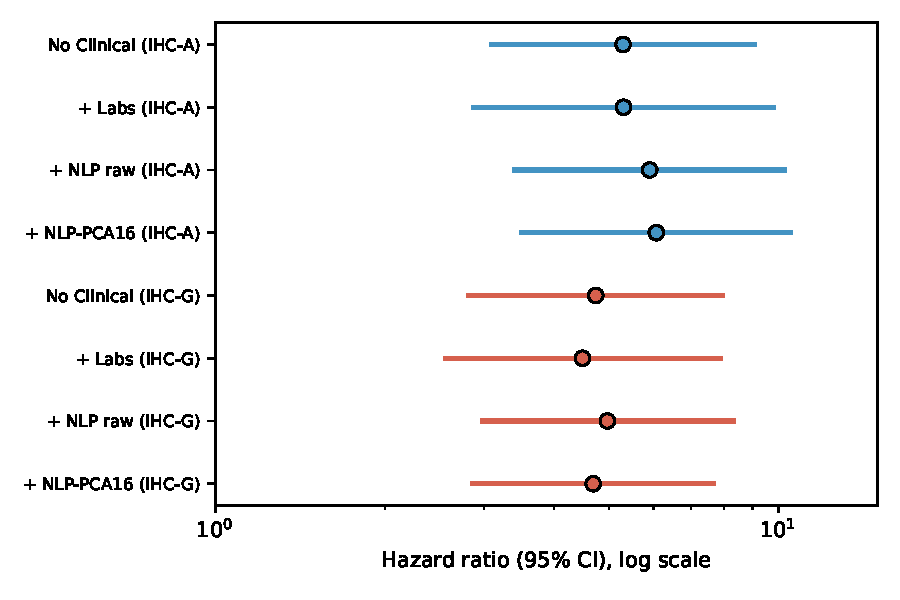
\includegraphics[width=0.48\textwidth]{figures/fig5c_cox_forest.pdf}}
  \hfill
  \subfloat[Integrated Brier Score]{%
    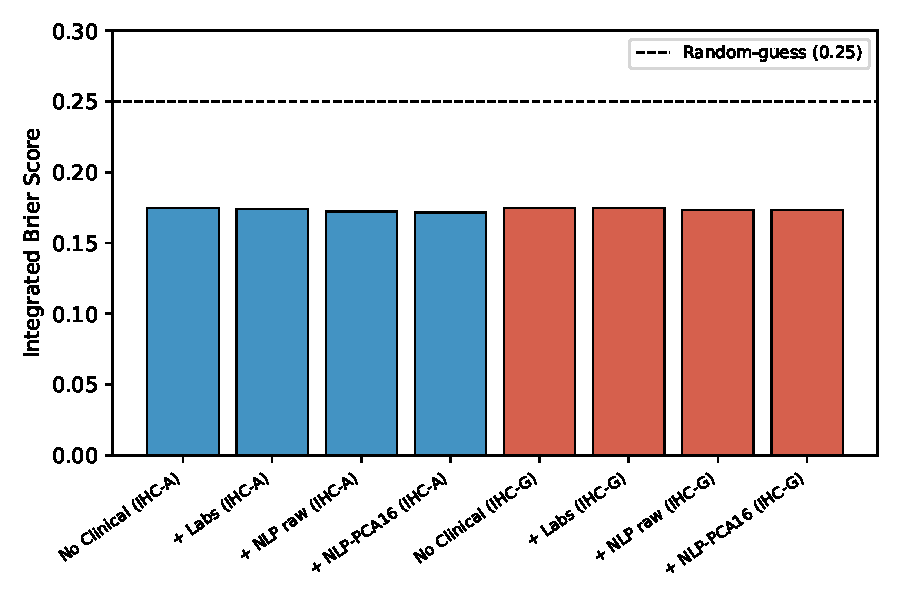
\includegraphics[width=0.48\textwidth]{figures/fig5d_ibs.pdf}}
  \caption{Survival analysis summary across clinical encoding strategies.
    (\textbf{A}) Harrell's C-index with bootstrap 95\% confidence intervals
    for IHC-A and IHC-G arms; differences between encoding strategies were
    not statistically significant (paired Wilcoxon $p > 0.05$).
    (\textbf{B}) Time-dependent AUC at 6, 12, and 18~months; NLP-encoded
    models show the largest advantage at 12--18~months.
    (\textbf{C}) Forest plot of multivariate Cox proportional hazards ratios
    for the fused risk score, adjusted for age, ECOG performance status,
    albumin, derived neutrophil-to-lymphocyte ratio, and liver metastases
    (all $p < 0.001$).
    (\textbf{D}) Integrated Brier Score (IBS) for each model; all values
    fall well below the 0.25 random-guess threshold (range
    0.172--0.175), indicating good calibration across all encoding
    strategies.}
  \label{fig:survival_summary}
\end{figure}

%% sections/discussion.tex — Step B10
\section{Discussion}
\label{sec:discussion}

In this study, we extended the DyAM multimodal attention framework with two
complementary contributions: a competitive (OvO) attention mechanism and an
NLP-based encoding of tabular clinical features, and evaluated both using
binary classification and survival endpoints.

The best-performing model, DyAM Rad+IHC-G+Gen+PDL1+NLP~raw, achieved
AUC~$= 0.813$ [95\%~CI: 0.753--0.874], placing it at the
``good-to-excellent'' discrimination threshold ($\text{AUC} > 0.80$) commonly
used in oncology decision support \cite{Vanguri2022}.
For context, this exceeds the single-source models evaluated in the same
cohort under the DyAM framework --- PD-L1~TPS alone (AUC~$= 0.720$) and TMB
alone (AUC~$= 0.616$) --- consistent with the modest discrimination reported
for these markers in the literature \cite{Rizvi2015,Reck2016}.
This confirms that multimodal fusion, augmented with NLP-encoded clinical
context, approaches the upper range of discrimination achievable with
currently available biomarkers in this disease setting.

Why does NLP encoding outperform raw numeric clinical features?
We propose that sentence embeddings capture non-linear interactions between
clinical variables --- for example, the combined prognostic implication of
advanced age, low albumin, and poor performance status --- that are not
explicitly represented in a 13-dimensional numeric vector.
The MiniLM-L6-v2 embedding space \cite{Reimers2019,Wang2020MiniLM} is
pretrained to place semantically similar sentences close together; patients
with similar overall clinical profiles are therefore mapped to nearby
embedding vectors even when no single numeric feature dominates.
Raw numeric encoding, by contrast, presents each variable to the attention
mechanism independently, requiring the model to learn these interactions
de novo from a relatively small training set.

The AUC improvements associated with NLP encoding ($+0.017$ to $+0.030$)
did not reach statistical significance under DeLong confidence interval
testing, as all CIs overlapped substantially.
This is best interpreted as a power limitation rather than an absent effect.
With $n = 247$, the 95\%~CI width for AUC is approximately $\pm 0.07$;
detecting a true $\Delta\text{AUC} \approx 0.02$ at 80\% power would require
approximately 950--1{,}250 patients (Supplementary Note~S3).
The directional consistency of the improvement across both the IHC-A and
IHC-G arms, and across raw and PCA-compressed NLP variants, supports a true
but modest effect size that is currently underpowered rather than null.

The survival analysis provides an important reframing of this finding.
While binary AUC improvements were modest and non-significant, multivariate
Cox regression showed that NLP-PCA16 achieved the highest hazard ratio in the
IHC-A arm (HR~$= 6.07$ vs.\ HR~$= 5.30$ for the no-clinical baseline), and
NLP raw achieved the highest hazard ratio in the IHC-G arm (HR~$= 4.97$ vs.\
HR~$= 4.74$), whereas numeric clinical labs provided no comparable
improvement in either arm.
Furthermore, the time-dependent AUC advantage of NLP encoding was
concentrated at 12 and 18~months ($+0.024$ and $+0.020$ in the IHC-A arm)
rather than at 6~months.
Taken together, these results suggest that NLP encoding of tabular clinical
features predominantly captures \emph{prognostic (time-to-event)} information
rather than \emph{predictive (binary response)} information --- a
distinction with direct implications for how such encodings should be
evaluated in future multimodal studies.

The OvO competitive attention mechanism matched the accuracy of the original
cooperative attention while using a substantially simpler parameterization.
An initial single-partition screen suggested a context-dependent pattern,
with OvO favoured in low-modality configurations
(up to $+3.27\%$ for PDL1+Gen) and the original model favoured as more
modalities were added; the overall best-performing single-partition
configuration (Rad+IHC-G+Gen+PDL1, AUC~$=0.8003$) used OvO attention.
A confirmatory repeated-seed analysis (5~seeds~$\times$~10-fold) placed the
two attention mechanisms within 0.011~AUC of each other at all four primary
benchmarks ($p \geq 0.17$), with OvO reaching a repeated-seed mean AUC of
$0.773$ versus $0.760$ for the cooperative model at the primary
configuration --- directionally favouring OvO, though the single-partition
``best'' configuration's rank relative to the cooperative model reversed
once averaged across seeds, underscoring the value of repeated-seed
evaluation over a single split.
Across all 21 configurations the repeated-seed data also reversed the
\emph{direction} of the context-dependence seen in the screen: OvO matched
or exceeded cooperative attention in 7 of 8 configurations fusing five or
more sources, but in only 5 of 9 configurations with two to four sources,
where the spread between the two mechanisms was several times larger.
A competitive one-vs-others weighting is plausibly better conditioned when
many partially redundant sources compete, whereas with few sources the
comparison against the mean of the remaining modalities is estimated from
one or two values and becomes unstable; we note, however, that the effect
sizes involved ($\leq 0.018$~AUC) sit below the seed-to-seed variability, so
this remains a hypothesis generated by the data rather than a tested claim.
When combined with NLP-clinical encoding, OvO reproduced the identical
fusion-dependent improvement pattern seen in the primary NLP-clinical
analysis (improvement in the same 15 of 21 configurations, decline in the
same six single-modality configurations), reaching AUC~$=0.782$ at the
primary benchmark under the repeated-seed protocol (repeated-seed
NLP-clinical confirmation: $0.783$) and
AUC~$=0.8133$ under the single-partition protocol at the
Rad+IHC-A+Gen+TMB+PDL1 configuration --- the highest value observed under
either protocol in this study.
OvO's practical value lies in its simpler parameterization ---
$N$ independent per-modality scores compared against the mean of the
remaining modalities, rather than the $N \times N$ weight matrix required by
cooperative attention --- delivering matching accuracy, and its improvement
pattern under NLP-clinical encoding generalises across both attention
mechanisms, indicating that the clinical-encoding intervention, not the
choice of attention mechanism, is the source of the observed gain.

From a clinical implementation perspective, NLP encoding of structured
clinical data offers practical advantages: encoding a patient profile
requires less than one second on CPU, requires no labelled clinical text,
and can be applied to any structured electronic health record (EHR) field
that can be rendered as a sentence.
This makes the approach readily transferable to other structured clinical
datasets without requiring a fine-tuned clinical language model.

Several limitations should be considered.
First, this was a single-institution retrospective cohort, which may limit
generalisability and introduce selection bias.
Second, the non-significant AUC improvement reflects the modest sample size
($n = 247$) rather than a definitive negative result, and larger
multi-institutional cohorts are needed to confirm the observed trends.
Third, the sentence encoder was applied in a zero-shot manner without
fine-tuning on NSCLC-specific clinical text, which may limit its sensitivity
to domain-specific terminology.
Finally, PD-L1 TPS was scored using the Sauter method in this cohort, which
may differ from the SP142 or 22C3 assays used at other institutions, and the
generalisability of PD-L1-derived features should be interpreted with this
in mind.

%% sections/conclusion.tex — Step B12
\section{Conclusions}
\label{sec:conclusion}

We extended the DyAM multimodal attention framework for ICI response
prediction in NSCLC with a competitive (OvO) attention mechanism and an
NLP-based encoding of structured clinical variables.
Under a repeated-seed evaluation protocol, OvO attention matched the
original cooperative attention at every primary benchmark configuration
(within 0.011~AUC, $p \geq 0.17$; AUC~$=0.773$ vs.\ $0.760$ at the primary
benchmark), offering a simpler, $N$-parameter alternative to the
$N \times N$ cooperative weight matrix without a measurable accuracy cost;
an initial single-partition screen had suggested a larger OvO advantage in
low-modality configurations (best single-partition AUC~$=0.800$, later
$0.8133$ when combined with NLP-clinical encoding), and averaging across
five independent CV partitions confirmed OvO's accuracy while showing this
particular single-partition margin does not reproduce exactly.
NLP encoding of clinical features using a general-purpose sentence
transformer consistently improved AUC over raw numeric encoding
(up to $\Delta\text{AUC} = +0.030$) and provided the strongest independent
prognostic value in survival analysis, with the highest Cox hazard ratios and
time-dependent AUC among all clinical encoding strategies, despite AUC
differences not reaching statistical significance at $n=247$.
This improvement was confirmed under repeated-seed evaluation (NLP
encoding exceeded numeric labs in 19 of 21 modality combinations) and
generalised across fusion mechanisms: combining NLP-clinical encoding with
OvO attention reproduced the same fusion-dependent gain, indicating that
the clinical-encoding strategy, rather than the choice of attention
mechanism, drives the improvement.
These findings suggest that sentence-embedding-based representations of
tabular clinical data are a practical and generalisable strategy for
multimodal biomarker discovery, robust to the underlying attention
architecture.
Validation in larger, multi-institutional cohorts is needed to confirm these
findings and to establish their clinical utility for treatment selection.


%% ── MDPI mandatory back-matter declarations ─────────────────────────────────
\authorcontributions{%
  Conceptualization, [F.A.] and [T.A.];
  methodology, [F.A.] and [S.A.];
  software, [F.A.];
  formal analysis, [F.A.];
  writing---original draft preparation, [F.A.];
  writing---review and editing, [S.A.] and [T.A.];
  supervision, [T.A.].
  All authors have read and agreed to the published version of the manuscript.
}

\funding{[FUNDING — e.g., This research received no external funding.]}

\institutionalreview{%
  This study was approved by the Institutional Review Board of [INSTITUTION]
  (Protocol No.~[IRB-NUMBER]).
}

\informedconsent{%
  Informed consent was obtained from all subjects involved in the study.
}

\dataavailability{%
  The code used in this study is available at
  \href{https://github.com/[REPO]}{https://github.com/[REPO]}.
  Patient-level data are subject to institutional data-sharing agreements
  and available upon reasonable request.
}

\conflictsofinterest{The authors declare no conflicts of interest.}

\bibliography{references}

\end{document}
